\documentclass[11pt, a4paper]{article}
\usepackage[utf8]{inputenc}
\usepackage[T1]{fontenc}
\usepackage[spanish, es-tabla]{babel}
\usepackage{newpxtext}
\usepackage{newpxmath}
\usepackage{microtype}
\usepackage[top=2.5cm, bottom=2.5cm, left=2.5cm, right=2.5cm]{geometry}
\usepackage{setspace}
\onehalfspacing
\usepackage{booktabs}
\usepackage{tabularx}
\usepackage{graphicx}
\usepackage{float}
\usepackage[font=small, labelfont=bf]{caption}
\usepackage{xcolor}
\definecolor{charcoal}{HTML}{2B2B2B}
\usepackage{titlesec}
\titleformat{\section}{\large\bfseries\color{black}}{\thesection.}{0.6em}{}
\titleformat{\subsection}{\normalsize\bfseries\color{black}}{\thesubsection.}{0.5em}{}
\titleformat{\subsubsection}{\normalsize\itshape\bfseries\color{black}}{\thesubsubsection.}{0.5em}{}
\usepackage[colorlinks=true, linkcolor=black, citecolor=black, urlcolor=charcoal]{hyperref}
\graphicspath{{figures/}{../figures/}}
\newsavebox{\reporttablebox}
\newcommand{\reporttable}[1]{%
  \begingroup\footnotesize
  \sbox{\reporttablebox}{#1}%
  \ifdim\wd\reporttablebox>\textwidth
    \resizebox{\textwidth}{!}{\usebox{\reporttablebox}}%
  \else
    \usebox{\reporttablebox}%
  \fi
  \endgroup
}
\title{Modelización estadística y evaluación probabilística del riesgo de incumplimiento crediticio: comparación entre modelos paramétricos y algoritmos de aprendizaje automático}
\author{Jean Paul Narváez González\\Universidad del Valle}
\date{18 de noviembre de 2026}
\begin{document}
\decimalpoint
\maketitle
\section*{Resumen}
Se estima la probabilidad de incumplimiento al mes siguiente a partir del historial de pago, los saldos y las características demográficas de 30.000 titulares de tarjetas de crédito en Taiwán en 2005. Se compara una regresión logística binomial, utilizada para la inferencia, con un árbol de decisión, un bosque aleatorio y XGBoost. La partición estratificada asigna el 70 \% a entrenamiento, el 15 \% a validación y el 15 \% a prueba. En prueba, XGBoost crudo obtuvo ROC-AUC de 0.7834 y precisión promedio de 0.5640. El ajuste isotónico, seleccionado en validación entre los calibradores, redujo el ECE uniforme de 0.0101 a 0.0097 y elevó el Brier de 0.1341 a 0.1346. El historial de pagos fue el bloque con mayor contribución predictiva en la ablación. En el escenario base, la pérdida esperada calibrada ascendió a 48,830,275 NTD y la simulación con probabilidades crudas a 49,306,232 NTD. La diferencia mide la sensibilidad a la calibración bajo supuestos de exposición y recuperación. El diseño transversal permite estimar asociaciones condicionales en la población estudiada.
\section{Introducción y Planteamiento del Problema}
La pregunta central es en qué medida las características demográficas, financieras y de comportamiento de pago permiten estimar el incumplimiento del mes siguiente. El objetivo inferencial es caracterizar asociaciones condicionales mediante un modelo paramétrico. El objetivo predictivo es contrastar discriminación y calidad probabilística fuera de muestra. La clasificación evalúa decisiones a un umbral concreto. La calibración permite interpretar la PD como frecuencia esperada y afecta directamente su uso en la estimación de pérdidas. La unidad de análisis es el titular de tarjeta.
\section{Datos, Auditoría de Calidad y Análisis Exploratorio}
El archivo UCI contiene 30\,000 clientes, 23 predictores, un identificador y la respuesta. La auditoría archivada registra cero faltantes, cero filas duplicadas completas y cero IDs duplicados. La exploración global registra 6\,636 incumplimientos (22.1200\%). La mediana del límite es 150,000 NTD en cumplidos y 90,000 NTD en incumplidos. La edad mediana es 34 en ambos grupos. El análisis exploratorio registra $V$ de Cramér de 0.4229 para \texttt{PAY\_0}, frente a $V\le 0.0731$ en demografía. Los 15 pares de facturas superan 0.7500 de correlación Pearson. Se agruparon los códigos de educación 0, 4, 5 y 6 en Otros y se incorporó el código 0 de estado civil a Otros. Los códigos de pago $-2$ y $0$ se conservaron sin atribuirles una interpretación económica específica. Se aplicaron pruebas de independencia $\chi^2$ y se reportó $V$ de Cramér como medida de magnitud. Las comparaciones de rangos emplearon Mann--Whitney bilateral con corrección por empates y continuidad. Para límite y edad se obtuvieron $p < 0.0001$ y $p = 0.3725$, respectivamente. Se examinaron correlaciones de Pearson y Spearman. Las pruebas marginales se interpretan de forma exploratoria, con cautela ante celdas escasas.
\section{Metodología de Validación y Prevención de Fuga de Datos}
La partición estratificada fija 70/15/15 (semilla 42) asignó 21\,000/4\,500/4\,500 clientes, con 4\,645/995/996 incumplimientos. Se excluyó \texttt{ID}. Los transformadores de \texttt{Pipeline} y \texttt{ColumnTransformer} se ajustaron dentro del entrenamiento correspondiente. La selección de especificación e hiperparámetros usó entrenamiento y pliegues estratificados internos. Validación sirvió para ordenar modelos, fijar umbrales y seleccionar y ajustar calibradores. Cada fila representa un cliente. Los seis meses son columnas de historial y el diseño carece de observaciones sucesivas de la variable objetivo por cliente. Por ello se utilizó una partición por cliente y se descartó la validación \emph{walk-forward}. Las evaluaciones individuales de prueba se reservaron a la comparación final y a la auditoría de calibración. La EDA histórica sí consultó agregados de la muestra completa, incluidas etiquetas, lo cual limita la independencia estricta de prueba.
\section{Modelización Paramétrica e Inferencia Estadística}
Se ajustó en statsmodels un GLM binomial con enlace logit. Los saldos se resumieron con la factura reciente y su diferencia frente al promedio de las cinco anteriores. M5 conserva la curvatura logarítmica del límite y las interacciones de \texttt{PAY\_0} con \texttt{LIMIT\_BAL} y \texttt{BILL\_AMT1}. Mejora AIC y BIC respecto a M0--M4 en las especificaciones archivadas. El LRT de omisión prueba cada término adicional condicionado a los demás, y los IC Wald son nominales tras la selección. La significancia de un coeficiente condicional depende de la parametrización. Para continuas, los OR corresponden a una unidad de la columna de diseño estandarizada, con los demás términos de diseño fijos. Variar el límite original mueve también su término logarítmico y la interacción. El OR principal de \texttt{PAY\_0} corresponde a límite y factura estandarizados iguales a cero. En ese punto, un incremento unitario en el código de septiembre multiplica las odds por 1.9288 (IC95: 1.8450 a 2.0164). Los diagnósticos del modelo base registraron 831 residuos de devianza con magnitud superior a 2 y 13 superiores a 3.

\subsection{Diagnóstico de la forma funcional}
El diagnóstico de Box--Tidwell examinó desviaciones de linealidad en el logit mediante términos $x \ln(x)$ y ajuste de Holm. Para el límite, el valor inicial de $p$ ajustado fue inferior a $0.0001$. En edad fue 0.9531. El resultado del ratio de pago fue sensible a la limitación de extremos: su $p$ ajustado pasó de un valor inferior a $0.0001$ a 0.6289 con tope en el cuantil 0.9900. Las conclusiones sobre los ratios se circunscriben al tratamiento de ceros, saldos negativos y denominadores inadmisibles del diagnóstico. La evaluación de influencia usa la distancia de Cook como diagnóstico de sensibilidad.

\subsection{Comparación de especificaciones}
\par\medskip\noindent\textbf{Especificaciones y contrastes anidados}

\noindent\reporttable{\begin{tabular}{lrrrrrrr}
\toprule
Modelo & k & AIC & BIC & Ref. & LR & gl & p LRT \\
\midrule
M0 & 23 & 19464.2 & 19647.1 &  &  &  &  \\
M1 & 24 & 19446.1 & 19637.0 & M0 & 20.1 & 1 & $< 0.0001$ \\
M2 & 25 & 19410.0 & 19608.8 & M1 & 38.1 & 1 & $< 0.0001$ \\
M3 & 26 & 19189.0 & 19395.8 & M2 & 223.0 & 1 & $< 0.0001$ \\
M4 & 25 & 19187.7 & 19386.6 & M1 & 260.4 & 1 & $< 0.0001$ \\
M5 & 26 & 19171.9 & 19378.7 & M4 & 17.8 & 1 & $< 0.0001$ \\
\bottomrule\end{tabular}}


\par\medskip\noindent\textbf{LRT de omisión en M5}

\noindent\reporttable{\begin{tabular}{lrrr}
\toprule
Término & LR & gl & p \\
\midrule
\texttt{LIMIT\_BAL\_log} & 17.8 & 1 & $< 0.0001$ \\
\texttt{PAY\_0 x LIMIT\_BAL} & 45.0 & 1 & $< 0.0001$ \\
\texttt{PAY\_0 x BILL\_AMT1} & 261.1 & 1 & $< 0.0001$ \\
\bottomrule\end{tabular}}


\par\medskip\noindent\textbf{VIF de las variables de facturación}

\noindent\reporttable{\begin{tabular}{lrrr}
\toprule
Variable & Seis saldos & M0 & M5 \\
\midrule
\texttt{BILL\_AMT1} & 13.9846 & 2.1459 & 2.4398 \\
\texttt{BILL\_AMT2} & 27.6025 &  &  \\
\texttt{BILL\_AMT3} & 25.0240 &  &  \\
\texttt{BILL\_AMT4} & 20.7126 &  &  \\
\texttt{BILL\_AMT5} & 24.2495 &  &  \\
\texttt{BILL\_AMT6} & 14.8861 &  &  \\
\texttt{BILL\_AMT1\_MINUS\_PREV5\_MEAN} &  & 1.7787 & 1.8317 \\
\bottomrule\end{tabular}}


\par\medskip\noindent\textbf{Inferencia Wald de M5}

\noindent\reporttable{\begin{tabular}{lrrrrrr}
\toprule
Término & Coef. & EE & p & OR & IC95 inf. & IC95 sup. \\
\midrule
\texttt{const} & -1.2579 & 0.0487 & $< 0.0001$ & 0.2843 & 0.2584 & 0.3127 \\
\texttt{SEX\_2} & -0.0903 & 0.0375 & 0.0161 & 0.9137 & 0.8489 & 0.9834 \\
\texttt{EDUCATION\_2} & -0.1218 & 0.0432 & 0.0048 & 0.8853 & 0.8134 & 0.9635 \\
\texttt{EDUCATION\_3} & -0.1831 & 0.0581 & 0.0016 & 0.8327 & 0.7431 & 0.9331 \\
\texttt{EDUCATION\_4} & -1.2458 & 0.2238 & $< 0.0001$ & 0.2877 & 0.1855 & 0.4461 \\
\texttt{MARRIAGE\_2} & -0.2003 & 0.0422 & $< 0.0001$ & 0.8185 & 0.7535 & 0.8890 \\
\texttt{MARRIAGE\_3} & -0.0811 & 0.1545 & 0.5998 & 0.9221 & 0.6812 & 1.2483 \\
\texttt{LIMIT\_BAL} & 0.0280 & 0.0463 & 0.5451 & 1.0284 & 0.9393 & 1.1260 \\
\texttt{AGE} & 0.0369 & 0.0208 & 0.0763 & 1.0376 & 0.9961 & 1.0808 \\
\texttt{BILL\_AMT1} & -0.2471 & 0.0374 & $< 0.0001$ & 0.7811 & 0.7259 & 0.8405 \\
\texttt{BILL\_AMT1\_MINUS\_PREV5\_MEAN} & -0.0308 & 0.0333 & 0.3553 & 0.9697 & 0.9084 & 1.0351 \\
\texttt{PAY\_AMT1} & -0.1292 & 0.0370 & 0.0005 & 0.8788 & 0.8174 & 0.9448 \\
\texttt{PAY\_AMT2} & -0.2306 & 0.0511 & $< 0.0001$ & 0.7940 & 0.7184 & 0.8777 \\
\bottomrule\end{tabular}}


\par\medskip\noindent\textbf{Inferencia Wald de M5 (continuación)}

\noindent\reporttable{\begin{tabular}{lrrrrrr}
\toprule
Término & Coef. & EE & p & OR & IC95 inf. & IC95 sup. \\
\midrule
\texttt{PAY\_AMT3} & -0.0416 & 0.0309 & 0.1785 & 0.9593 & 0.9029 & 1.0192 \\
\texttt{PAY\_AMT4} & -0.0466 & 0.0287 & 0.1045 & 0.9545 & 0.9023 & 1.0097 \\
\texttt{PAY\_AMT5} & -0.0358 & 0.0276 & 0.1949 & 0.9649 & 0.9140 & 1.0185 \\
\texttt{PAY\_AMT6} & -0.0608 & 0.0297 & 0.0408 & 0.9410 & 0.8877 & 0.9975 \\
\texttt{LIMIT\_BAL\_log} & -0.1805 & 0.0425 & $< 0.0001$ & 0.8348 & 0.7681 & 0.9073 \\
\texttt{PAY\_0} & 0.6569 & 0.0227 & $< 0.0001$ & 1.9288 & 1.8450 & 2.0164 \\
\texttt{PAY\_2} & 0.0211 & 0.0248 & 0.3949 & 1.0213 & 0.9729 & 1.0721 \\
\texttt{PAY\_3} & 0.0726 & 0.0270 & 0.0072 & 1.0753 & 1.0199 & 1.1338 \\
\texttt{PAY\_4} & 0.0574 & 0.0299 & 0.0546 & 1.0591 & 0.9989 & 1.1229 \\
\texttt{PAY\_5} & 0.0227 & 0.0322 & 0.4809 & 1.0230 & 0.9604 & 1.0897 \\
\texttt{PAY\_6} & 0.0310 & 0.0264 & 0.2399 & 1.0315 & 0.9795 & 1.0862 \\
\texttt{PAY\_0 x LIMIT\_BAL} & -0.1309 & 0.0194 & $< 0.0001$ & 0.8773 & 0.8446 & 0.9112 \\
\texttt{PAY\_0 x BILL\_AMT1} & 0.3742 & 0.0250 & $< 0.0001$ & 1.4538 & 1.3842 & 1.5269 \\
\bottomrule\end{tabular}}


\begin{figure}[htbp]\centering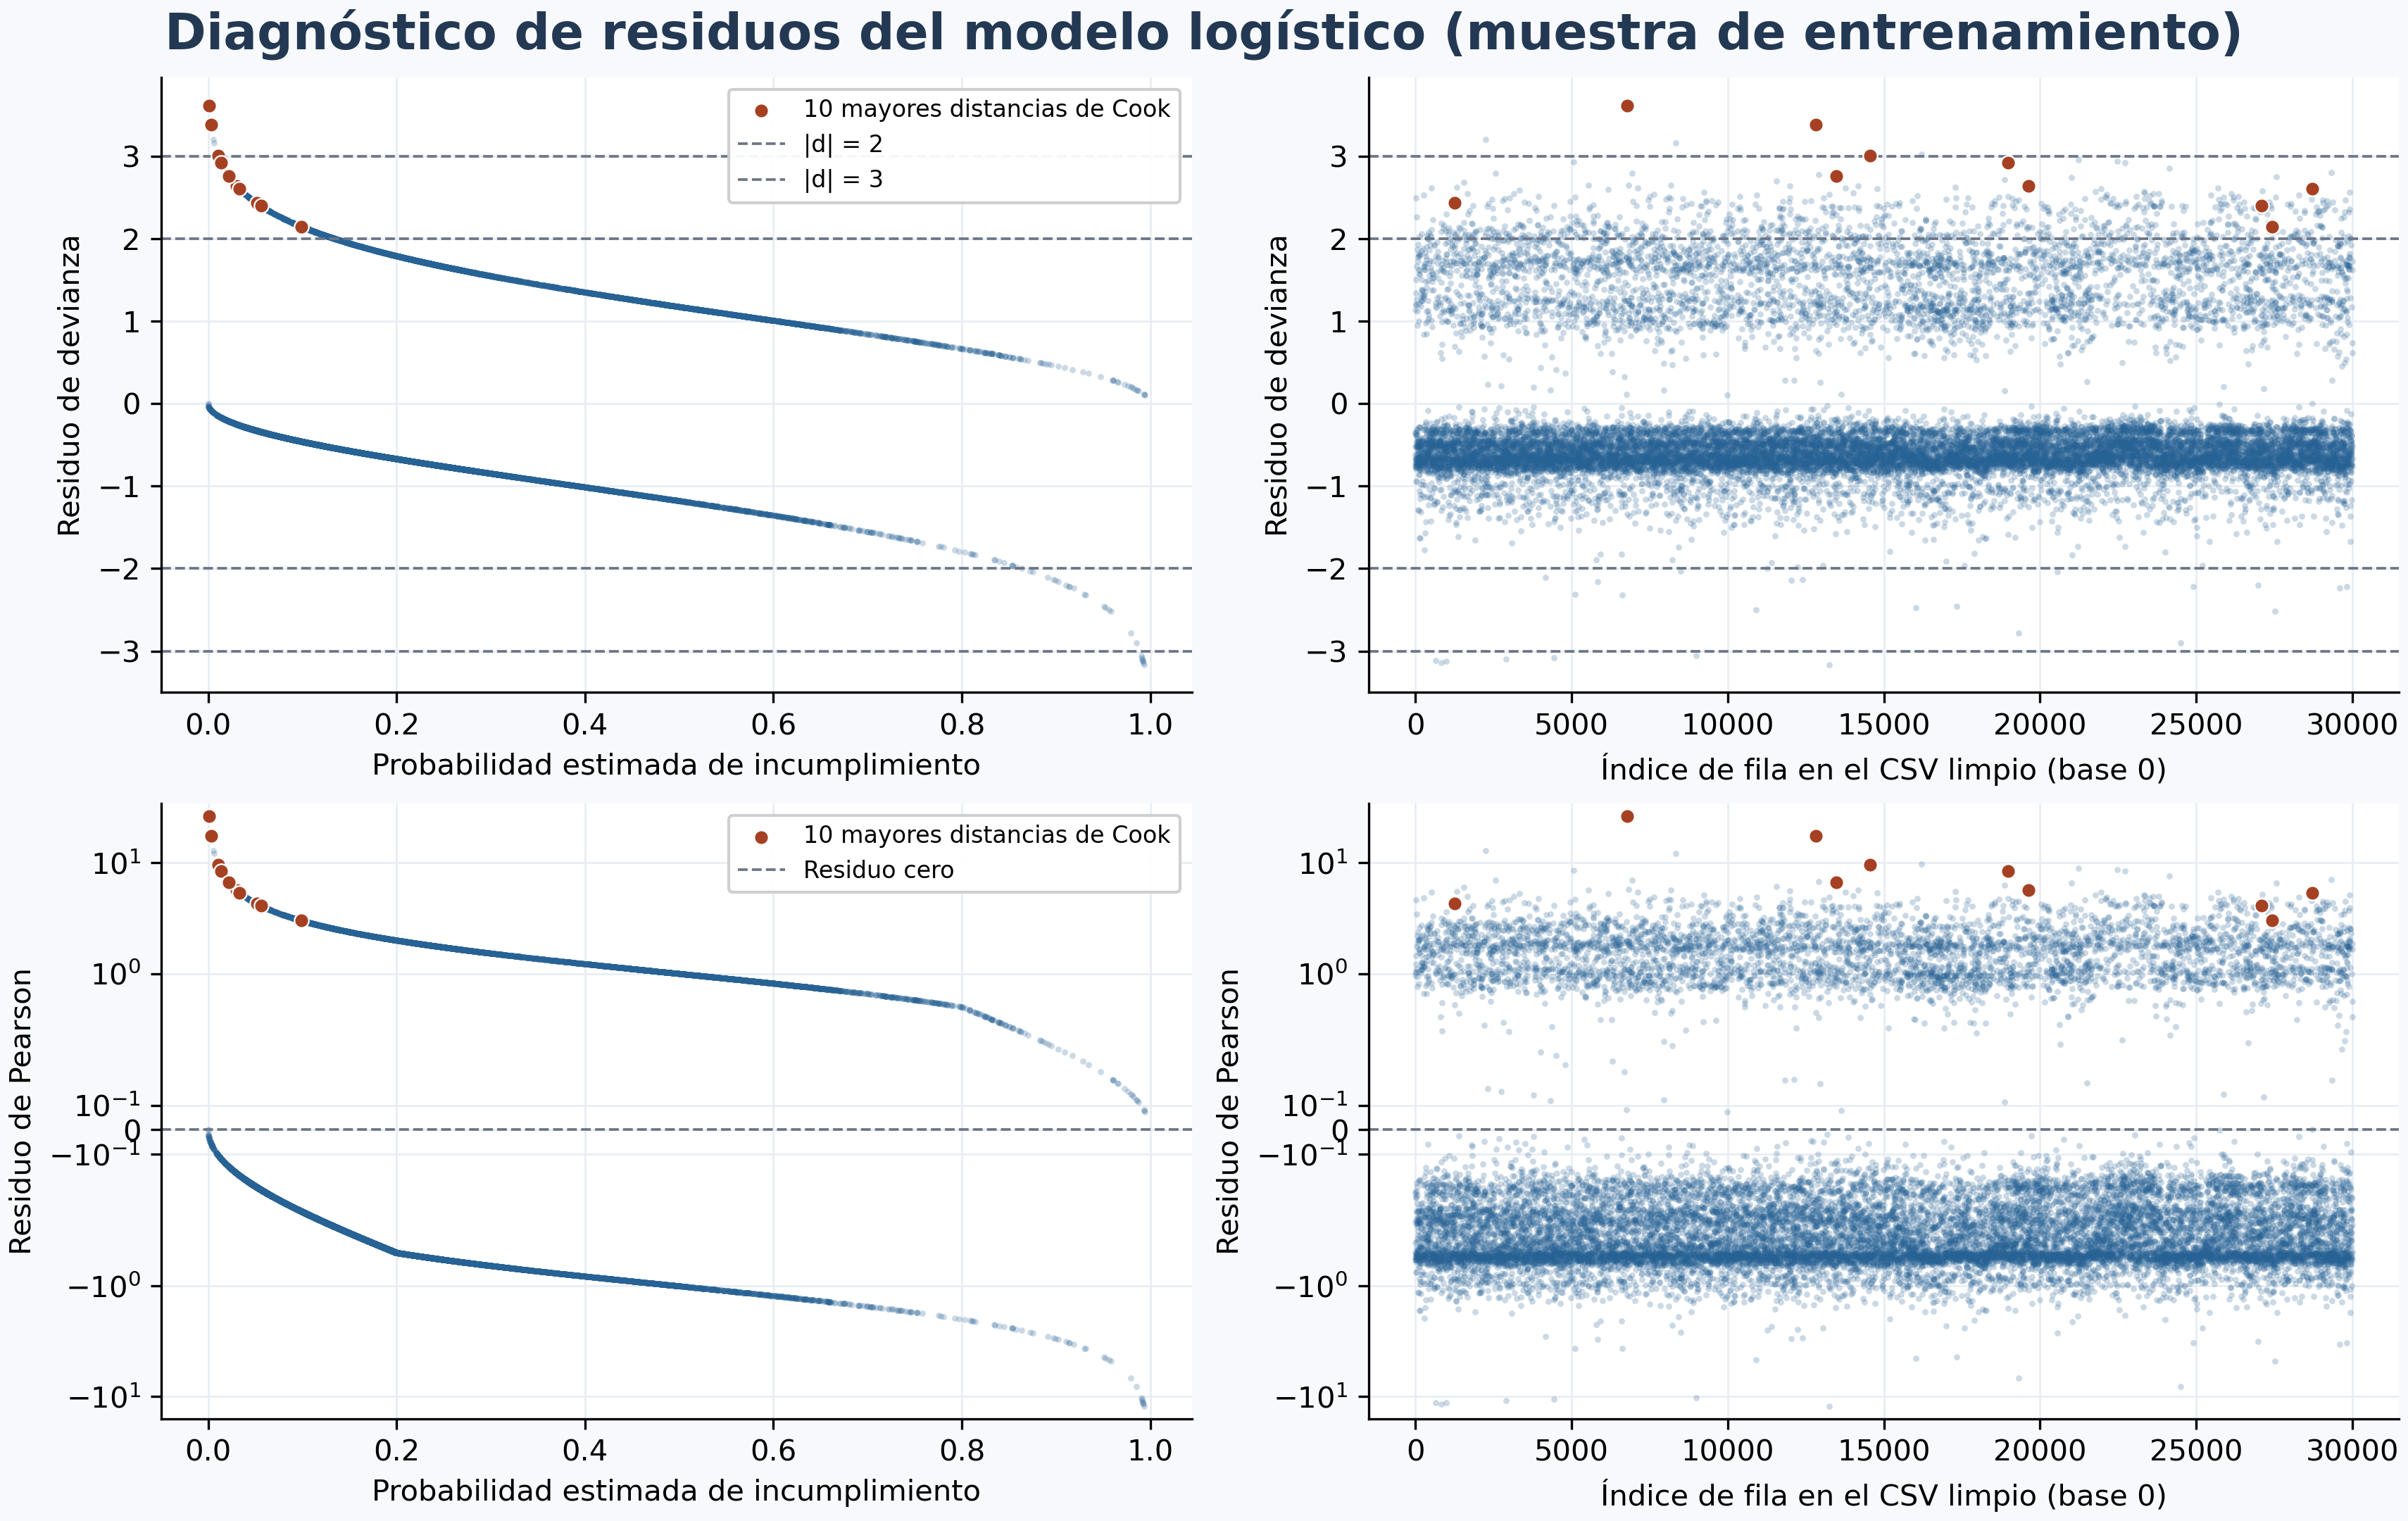
\includegraphics[width=\linewidth,height=.68\textheight,keepaspectratio]{05_logistic_diagnostics_residuals.png}\caption{Diagnóstico de residuos del modelo base.}\end{figure}

\begin{figure}[htbp]\centering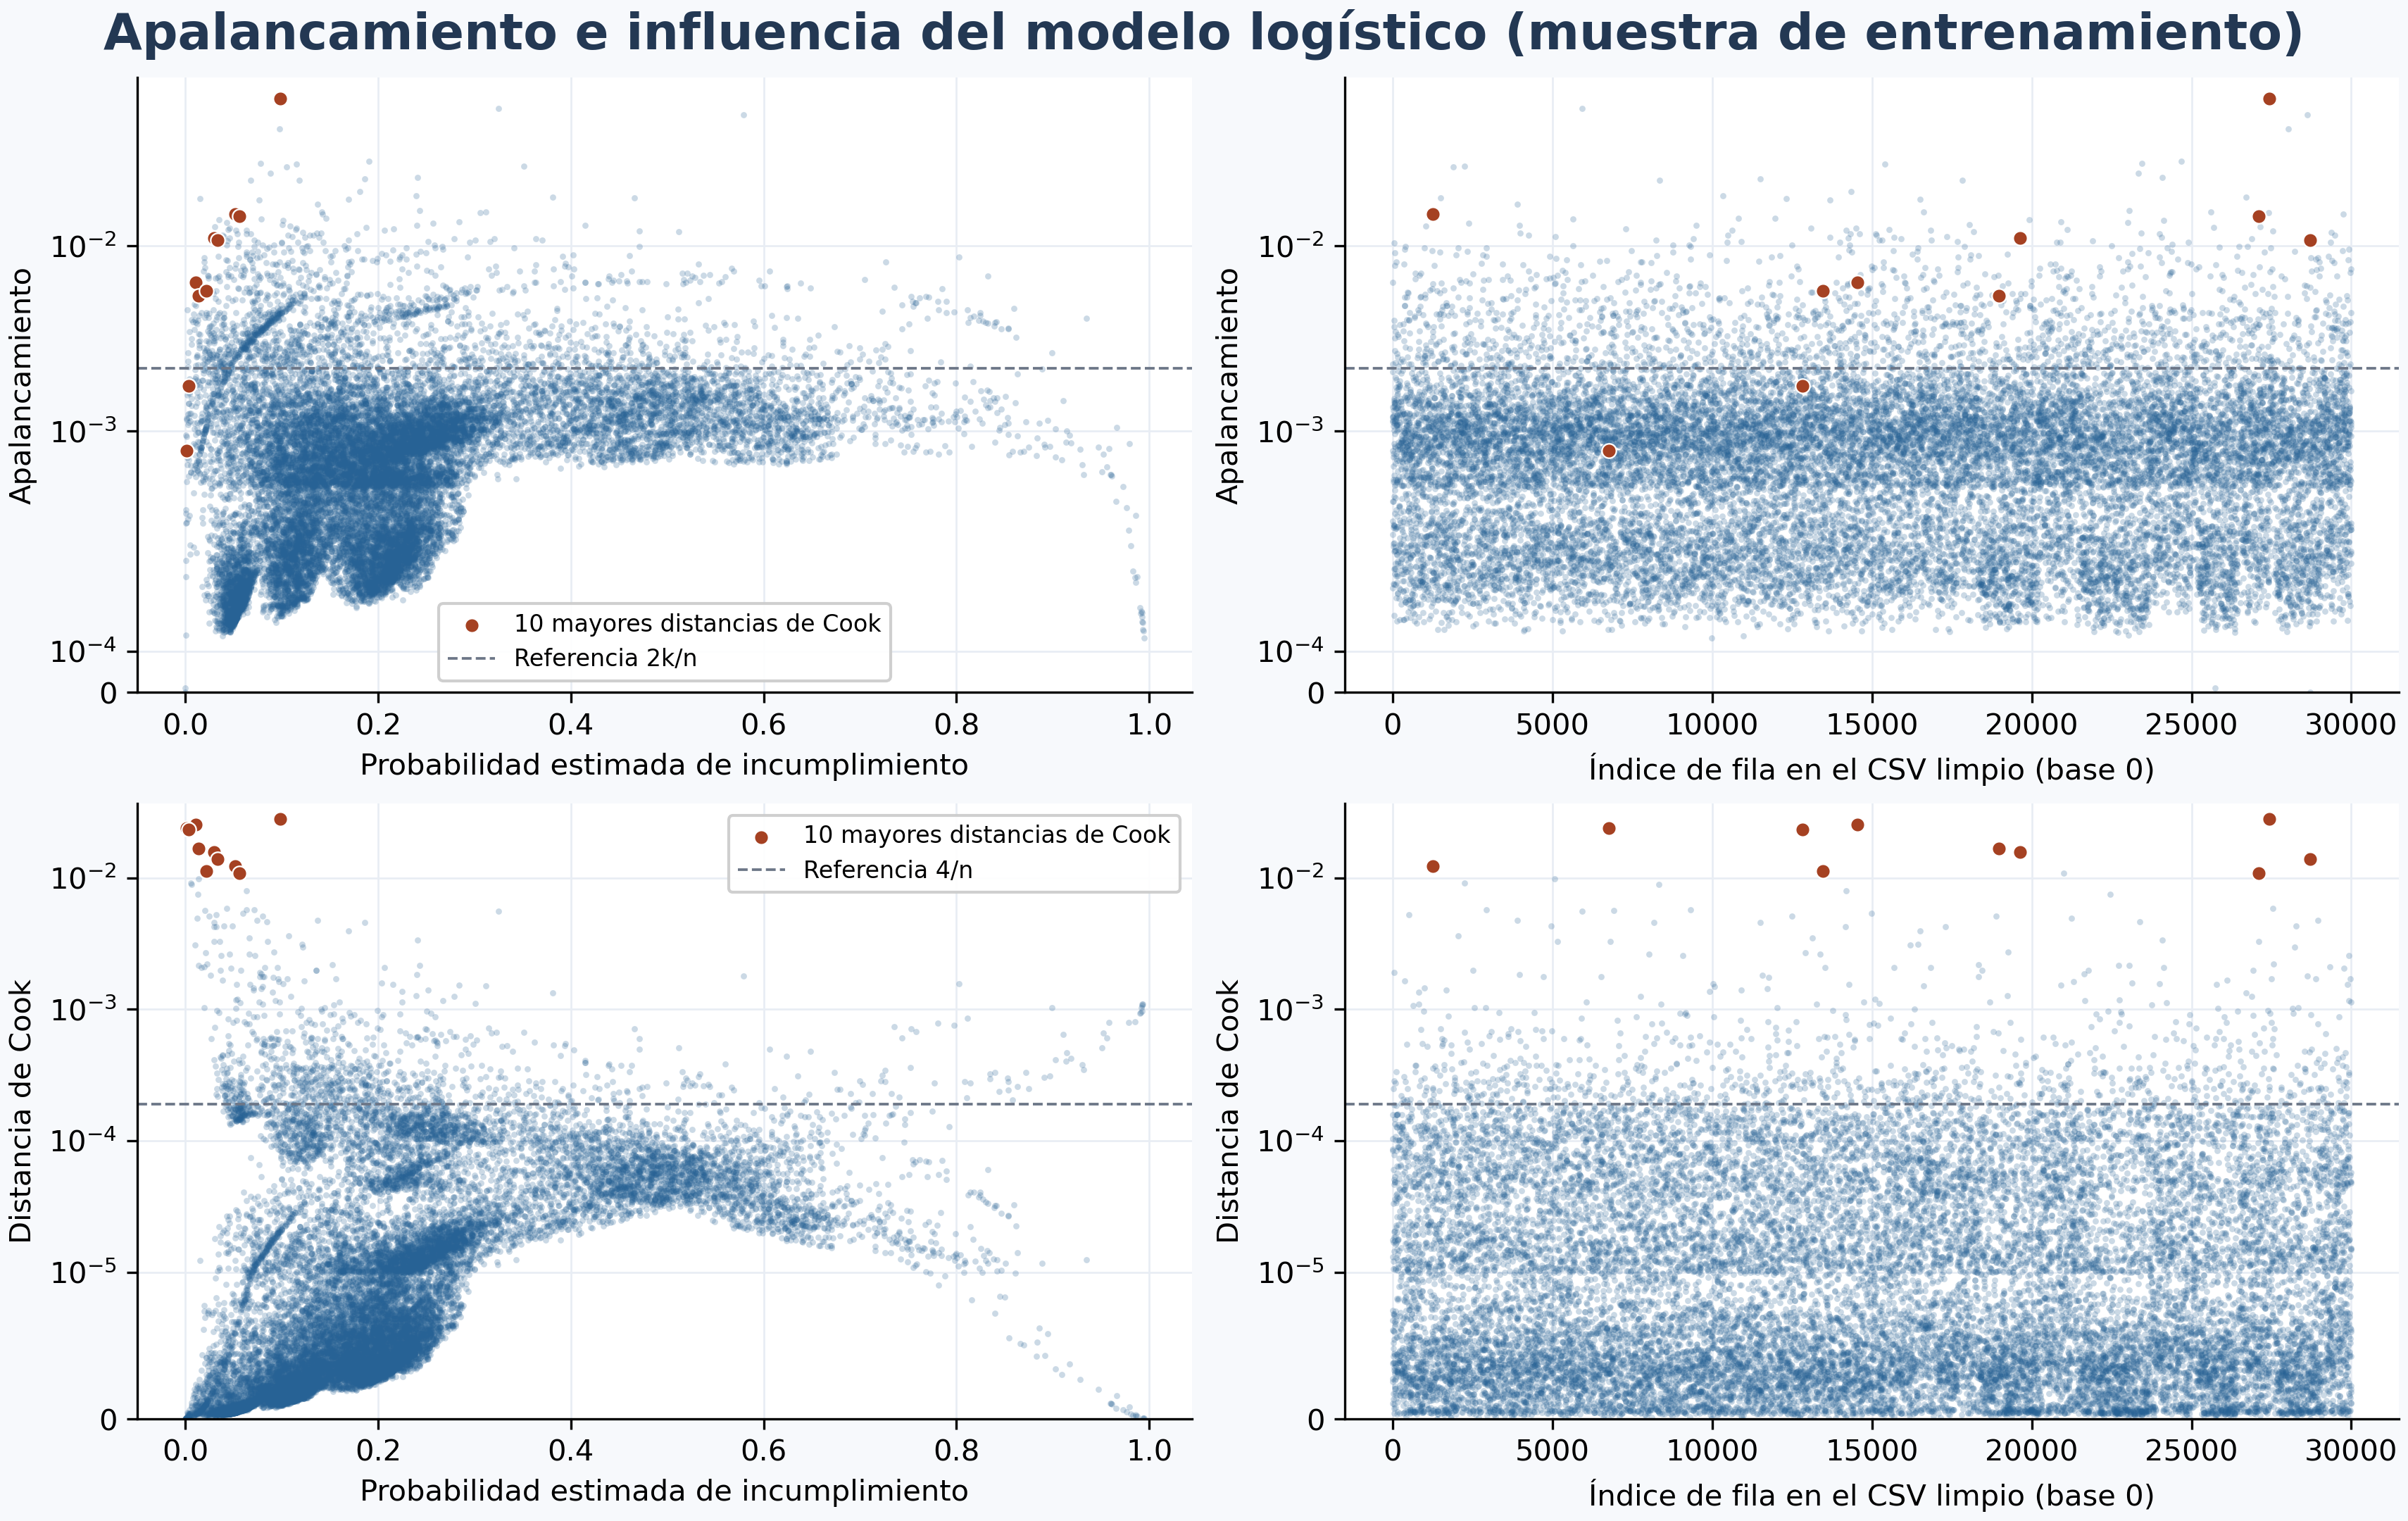
\includegraphics[width=\linewidth,height=.68\textheight,keepaspectratio]{06_logistic_influence_cooks.png}\caption{Influencia de observaciones y distancia de Cook.}\end{figure}

\clearpage
\section{Algoritmos de Aprendizaje Automático y Estudio de Ablación}
El árbol y el bosque se ajustaron por búsqueda interna estratificada. La comparación en prueba incluyó XGBoost, entrenado con 16 candidatos y cinco pliegues internos, junto con el árbol, el bosque y M5. El análisis de importancia archivado incluye HistGradientBoosting como referencia en validación. El liderazgo de XGBoost crudo en validación justificó su uso en ablación. En prueba, la incertidumbre del contraste exploratorio pareado con el bosque incluye cero, por lo cual el orden observado ofrece evidencia limitada de superioridad poblacional. AP es la precisión promedio y su referencia sin discriminación es $996/4500$.

\subsection{Discriminación y desempeño a umbral fijo}
Las métricas ROC-AUC y AP para las probabilidades crudas se presentan junto con las calibradas en la sección siguiente. El contraste de ROC-AUC utiliza remuestreo bootstrap pareado y estratificado de las predicciones, con 1\,000 réplicas. F1 se reporta al corte fijo y con el corte de Youden estimado en validación.
\begin{table}[H]
\centering
\caption{F1 por regla de clasificación en prueba}
\reporttable{\begin{tabular}{llrr}
\toprule
Modelo & Regla & Umbral & F1 \\
\midrule
Logística M5 & 0.5000 & 0.5000 & 0.4177 \\
Logística M5 & Youden val & 0.2891 & 0.5132 \\
Árbol & 0.5000 & 0.5000 & 0.4560 \\
Árbol & Youden val & 0.2269 & 0.5128 \\
Random Forest & 0.5000 & 0.5000 & 0.4578 \\
Random Forest & Youden val & 0.2350 & 0.5404 \\
XGBoost & 0.5000 & 0.5000 & 0.4640 \\
XGBoost & Youden val & 0.2078 & 0.5354 \\
\bottomrule
\end{tabular}}
\end{table}

\par\medskip\noindent\textbf{Contraste ROC-AUC pareado (bootstrap estratificado, 1\,000 réplicas)}

\noindent\reporttable{\begin{tabular}{lrrrr}
\toprule
Comparación & Diferencia & IC95 inf. & IC95 sup. & p bilateral \\
\midrule
XGBoost vs. bosque & 0.0017 & -0.0019 & 0.0054 & 0.3576 \\
\bottomrule\end{tabular}}


\par\medskip\noindent\textbf{Ablación en prueba}

\noindent\reporttable{\begin{tabular}{lrrrrr}
\toprule
modelo & variante & ROC-AUC & PR-AUC (AP) & Log Loss & F1 \\
\midrule
prob\_xgb & A & 0.5782 & 0.2668 & 0.5218 & 0.0000 \\
prob\_xgb & B & 0.7440 & 0.5303 & 0.4427 & 0.4515 \\
prob\_xgb & C & 0.7319 & 0.4494 & 0.4675 & 0.2691 \\
prob\_xgb & D & 0.7834 & 0.5640 & 0.4271 & 0.4640 \\
prob\_xgb & sin A & 0.7801 & 0.5540 & 0.4299 & 0.4551 \\
prob\_xgb & sin B & 0.7344 & 0.4477 & 0.4664 & 0.2605 \\
prob\_xgb & sin C & 0.7575 & 0.5505 & 0.4386 & 0.4566 \\
prob\_logreg & A & 0.5586 & 0.2596 & 0.5235 & 0.0000 \\
prob\_logreg & B & 0.7037 & 0.4832 & 0.4754 & 0.3384 \\
prob\_logreg & C & 0.6469 & 0.3273 & 0.5094 & 0.0000 \\
prob\_logreg & D & 0.7294 & 0.5021 & 0.4606 & 0.4177 \\
prob\_logreg & sin A & 0.7200 & 0.4952 & 0.4643 & 0.4178 \\
prob\_logreg & sin B & 0.6583 & 0.3322 & 0.5049 & 0.0080 \\
prob\_logreg & sin C & 0.7090 & 0.4964 & 0.4719 & 0.3512 \\
\bottomrule\end{tabular}}


\par\medskip\noindent\textbf{Cambios en discriminación por bloque}

\noindent\reporttable{\begin{tabular}{lrrrr}
\toprule
modelo & bloque & contraste & $\Delta$ ROC-AUC & $\Delta$ PR-AUC (AP) \\
\midrule
prob\_xgb & A & D - bloque aislado & 0.2052 & 0.2973 \\
prob\_xgb & A & D - modelo sin bloque & 0.0033 & 0.0101 \\
prob\_xgb & B & D - bloque aislado & 0.0394 & 0.0337 \\
prob\_xgb & B & D - modelo sin bloque & 0.0491 & 0.1163 \\
prob\_xgb & C & D - bloque aislado & 0.0516 & 0.1146 \\
prob\_xgb & C & D - modelo sin bloque & 0.0259 & 0.0135 \\
prob\_logreg & A & D - bloque aislado & 0.1708 & 0.2425 \\
prob\_logreg & A & D - modelo sin bloque & 0.0094 & 0.0070 \\
prob\_logreg & B & D - bloque aislado & 0.0257 & 0.0190 \\
prob\_logreg & B & D - modelo sin bloque & 0.0711 & 0.1699 \\
prob\_logreg & C & D - bloque aislado & 0.0825 & 0.1748 \\
prob\_logreg & C & D - modelo sin bloque & 0.0204 & 0.0058 \\
\bottomrule\end{tabular}}


A agrupa demografía, B los estados \texttt{PAY\_0}, \texttt{PAY\_2} a \texttt{PAY\_6}, C límite, facturas y montos pagados, y D todos los predictores. B presenta la mayor señal como bloque aislado entre A, B y C, y su retiro de D produce la mayor caída de AP y ROC-AUC en ambos modelos. Financieramente, el atraso reciente y su persistencia informan sobre dificultades de pago ya observadas dentro del ciclo de crédito. El experimento cuantifica valor predictivo condicional al diseño, sin identificar el efecto de una intervención sobre el atraso.

\begin{figure}[htbp]\centering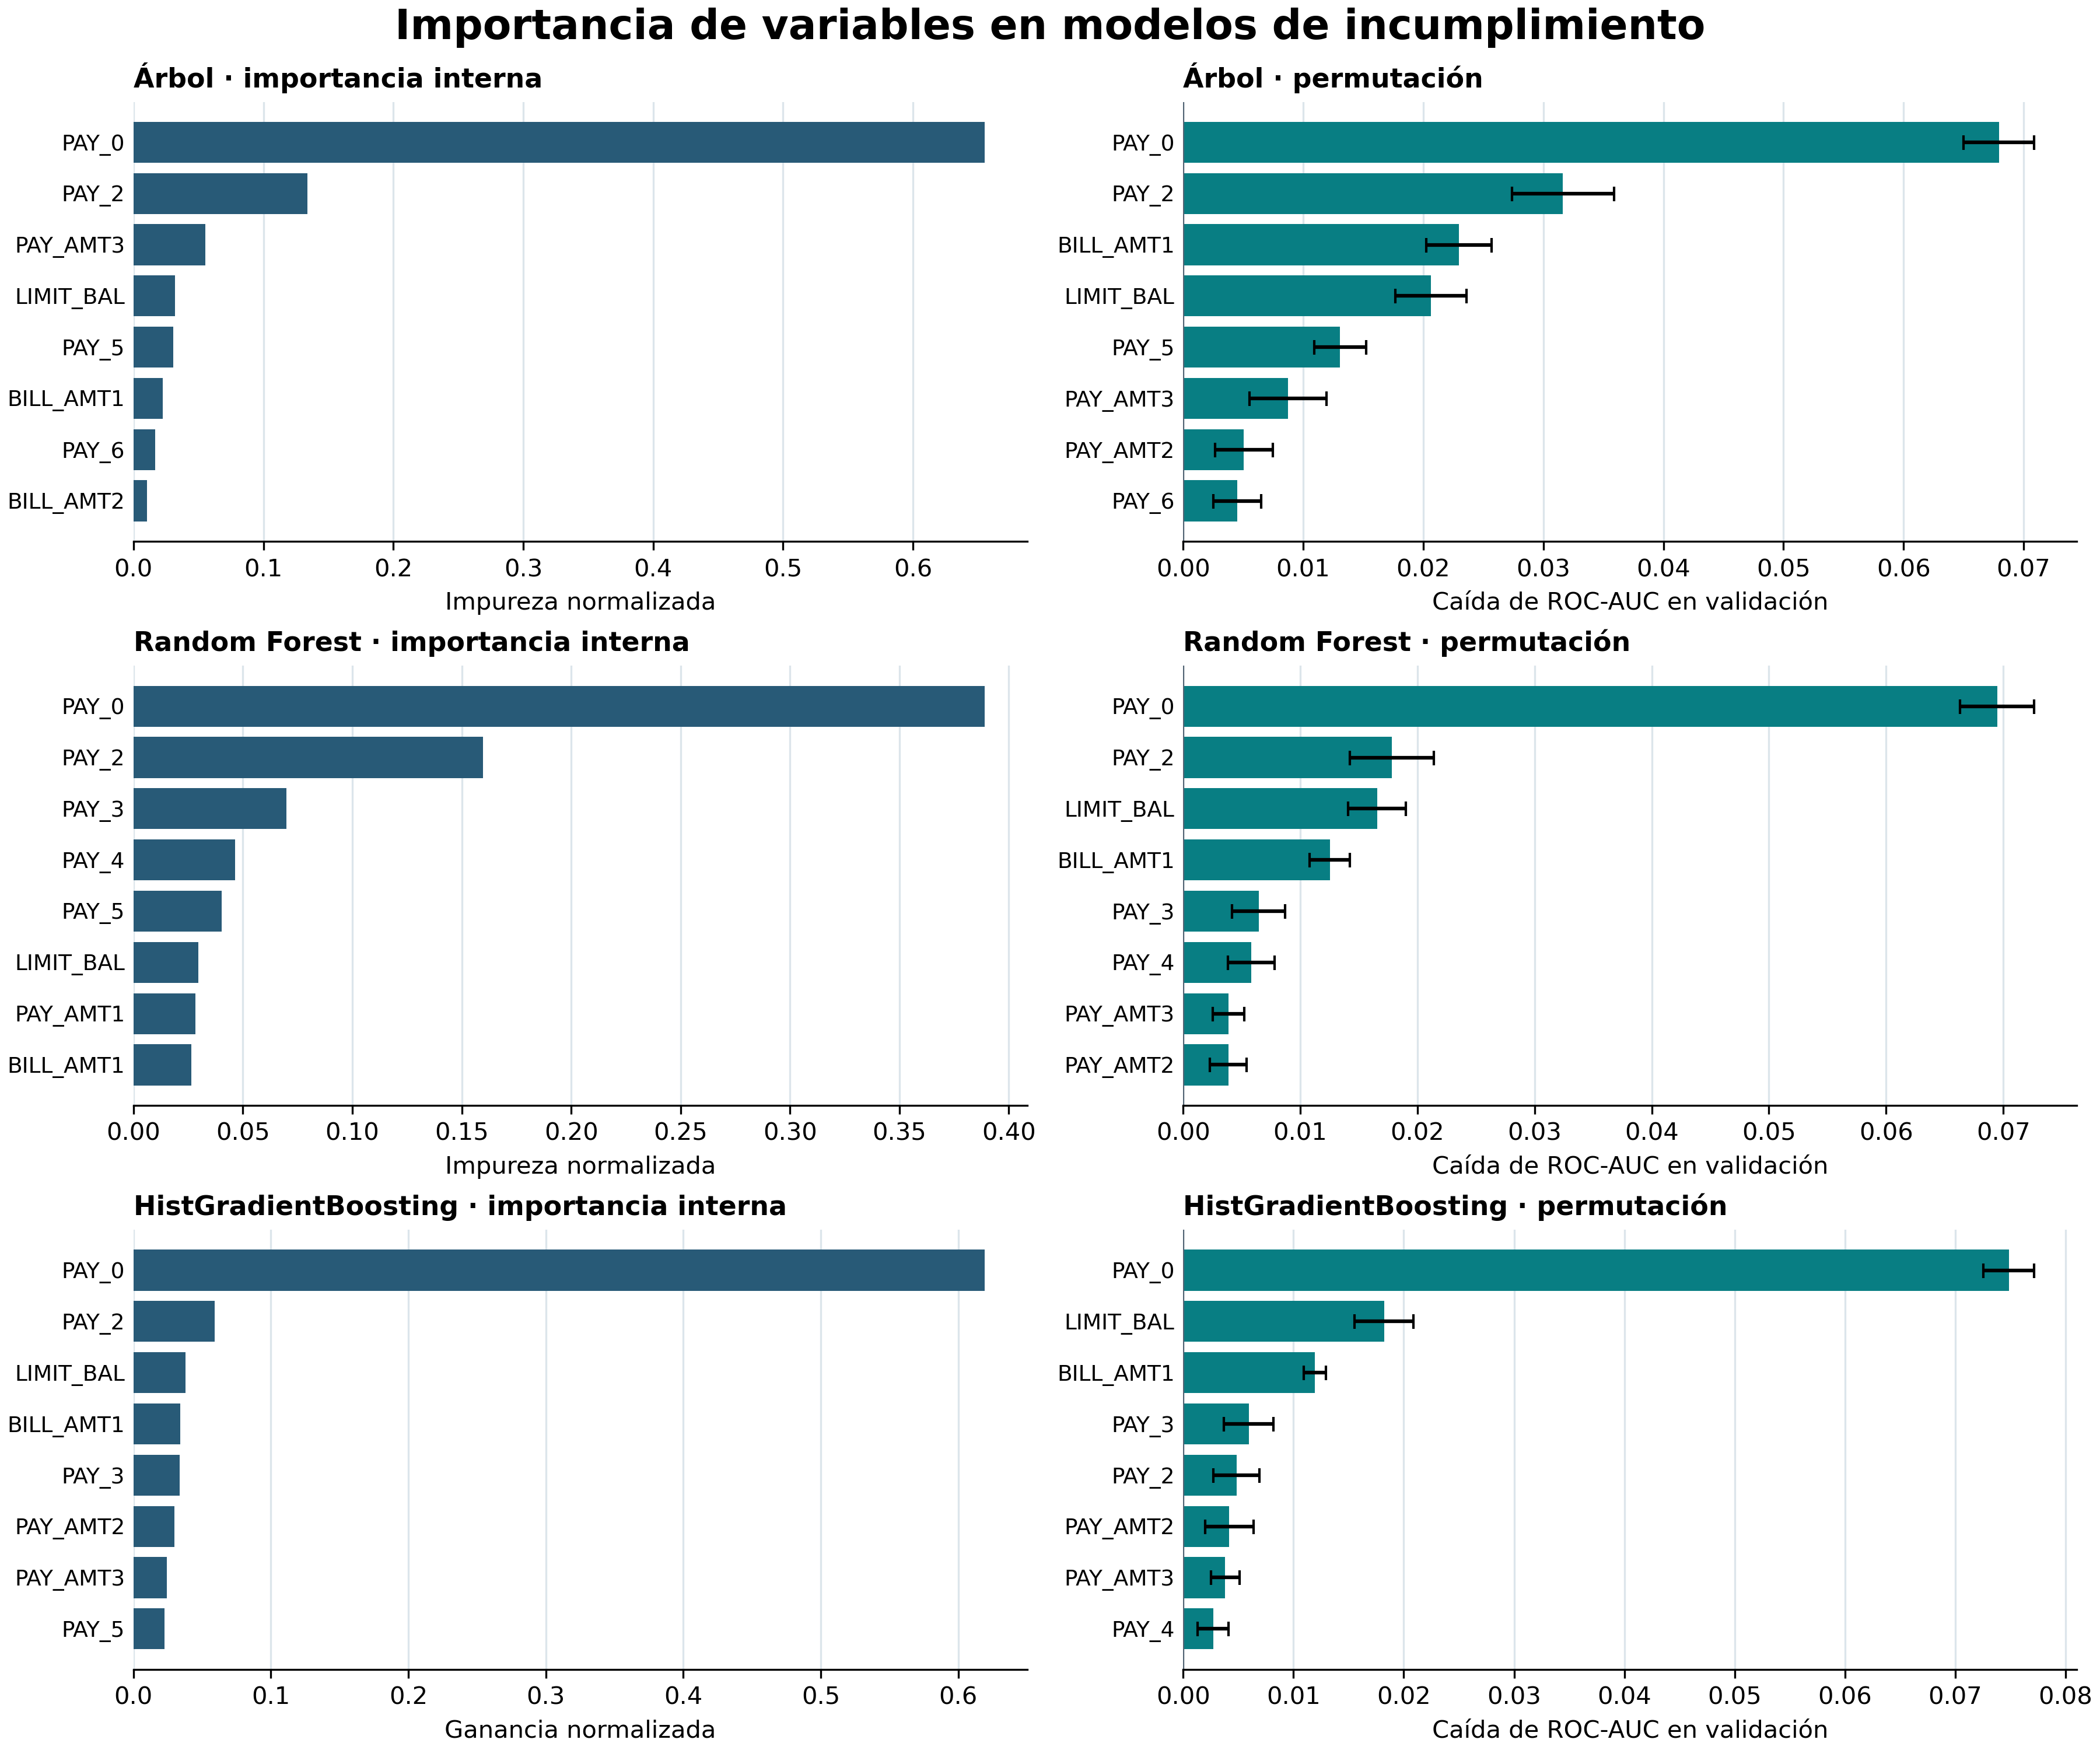
\includegraphics[width=\linewidth,height=.68\textheight,keepaspectratio]{07_ml_feature_importance.png}\caption{Importancia de predictores en validación para árbol, bosque e HistGradientBoosting.}\end{figure}

\begin{figure}[htbp]\centering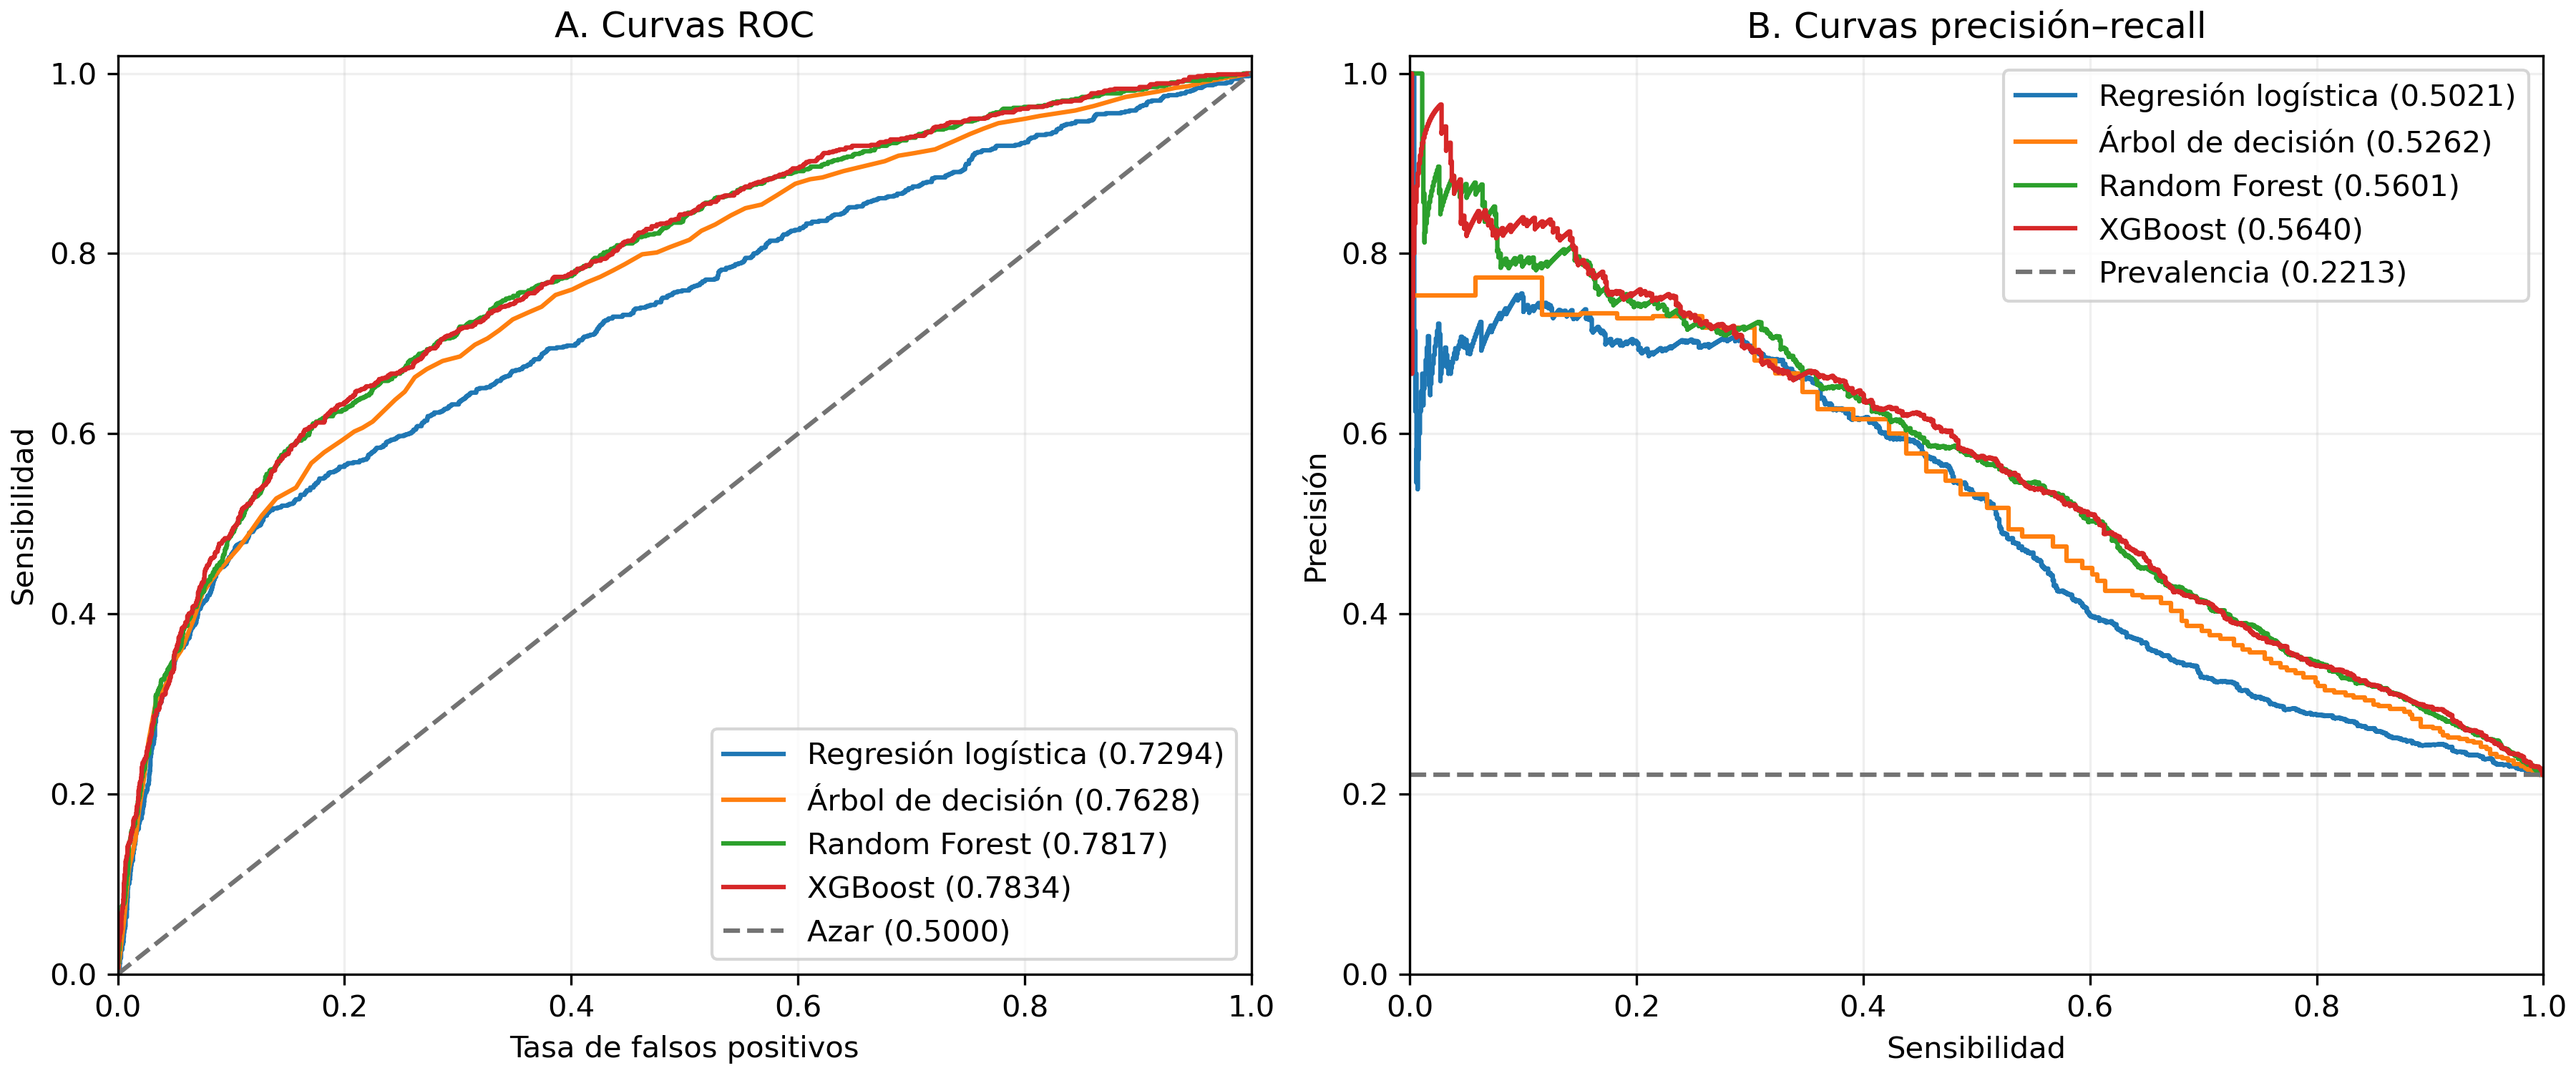
\includegraphics[width=\linewidth,height=.68\textheight,keepaspectratio]{08_test_roc_pr_curves.png}\caption{Curvas ROC y precisión-recall en prueba.}\end{figure}

\begin{figure}[htbp]\centering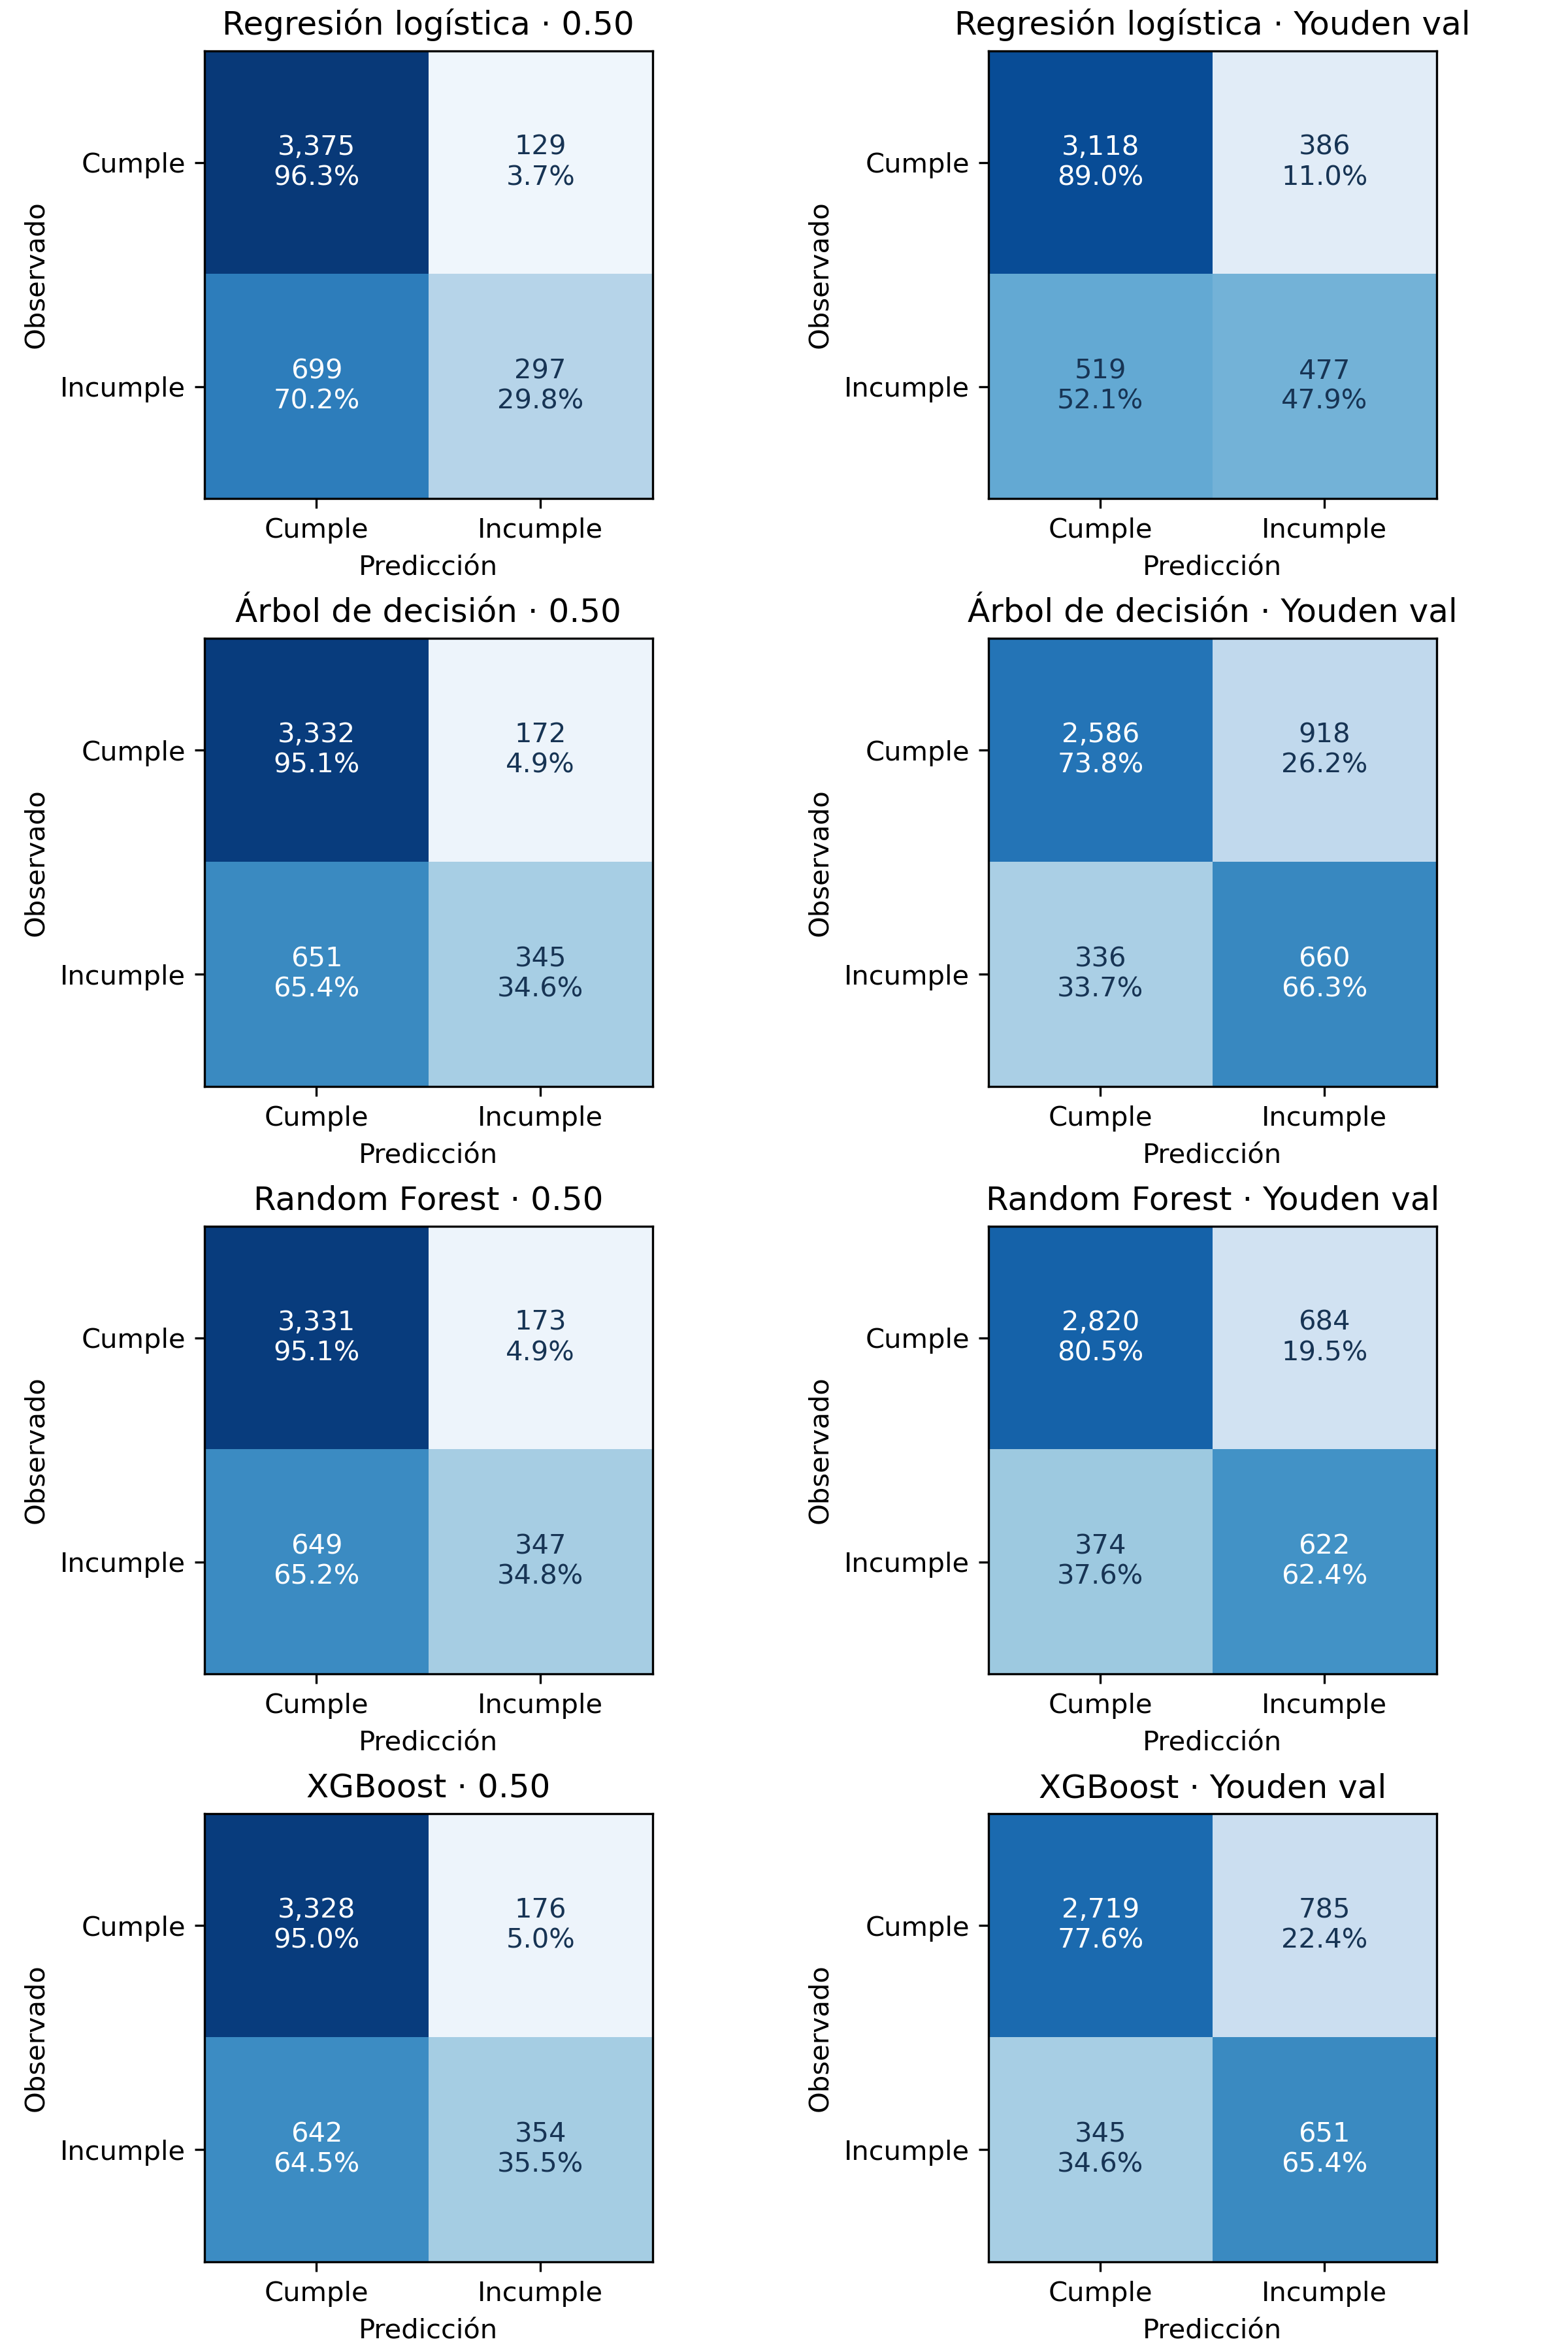
\includegraphics[width=\linewidth,height=.68\textheight,keepaspectratio]{09_test_confusion_matrices.png}\caption{Matrices de confusión normalizadas en prueba.}\end{figure}

\begin{figure}[htbp]\centering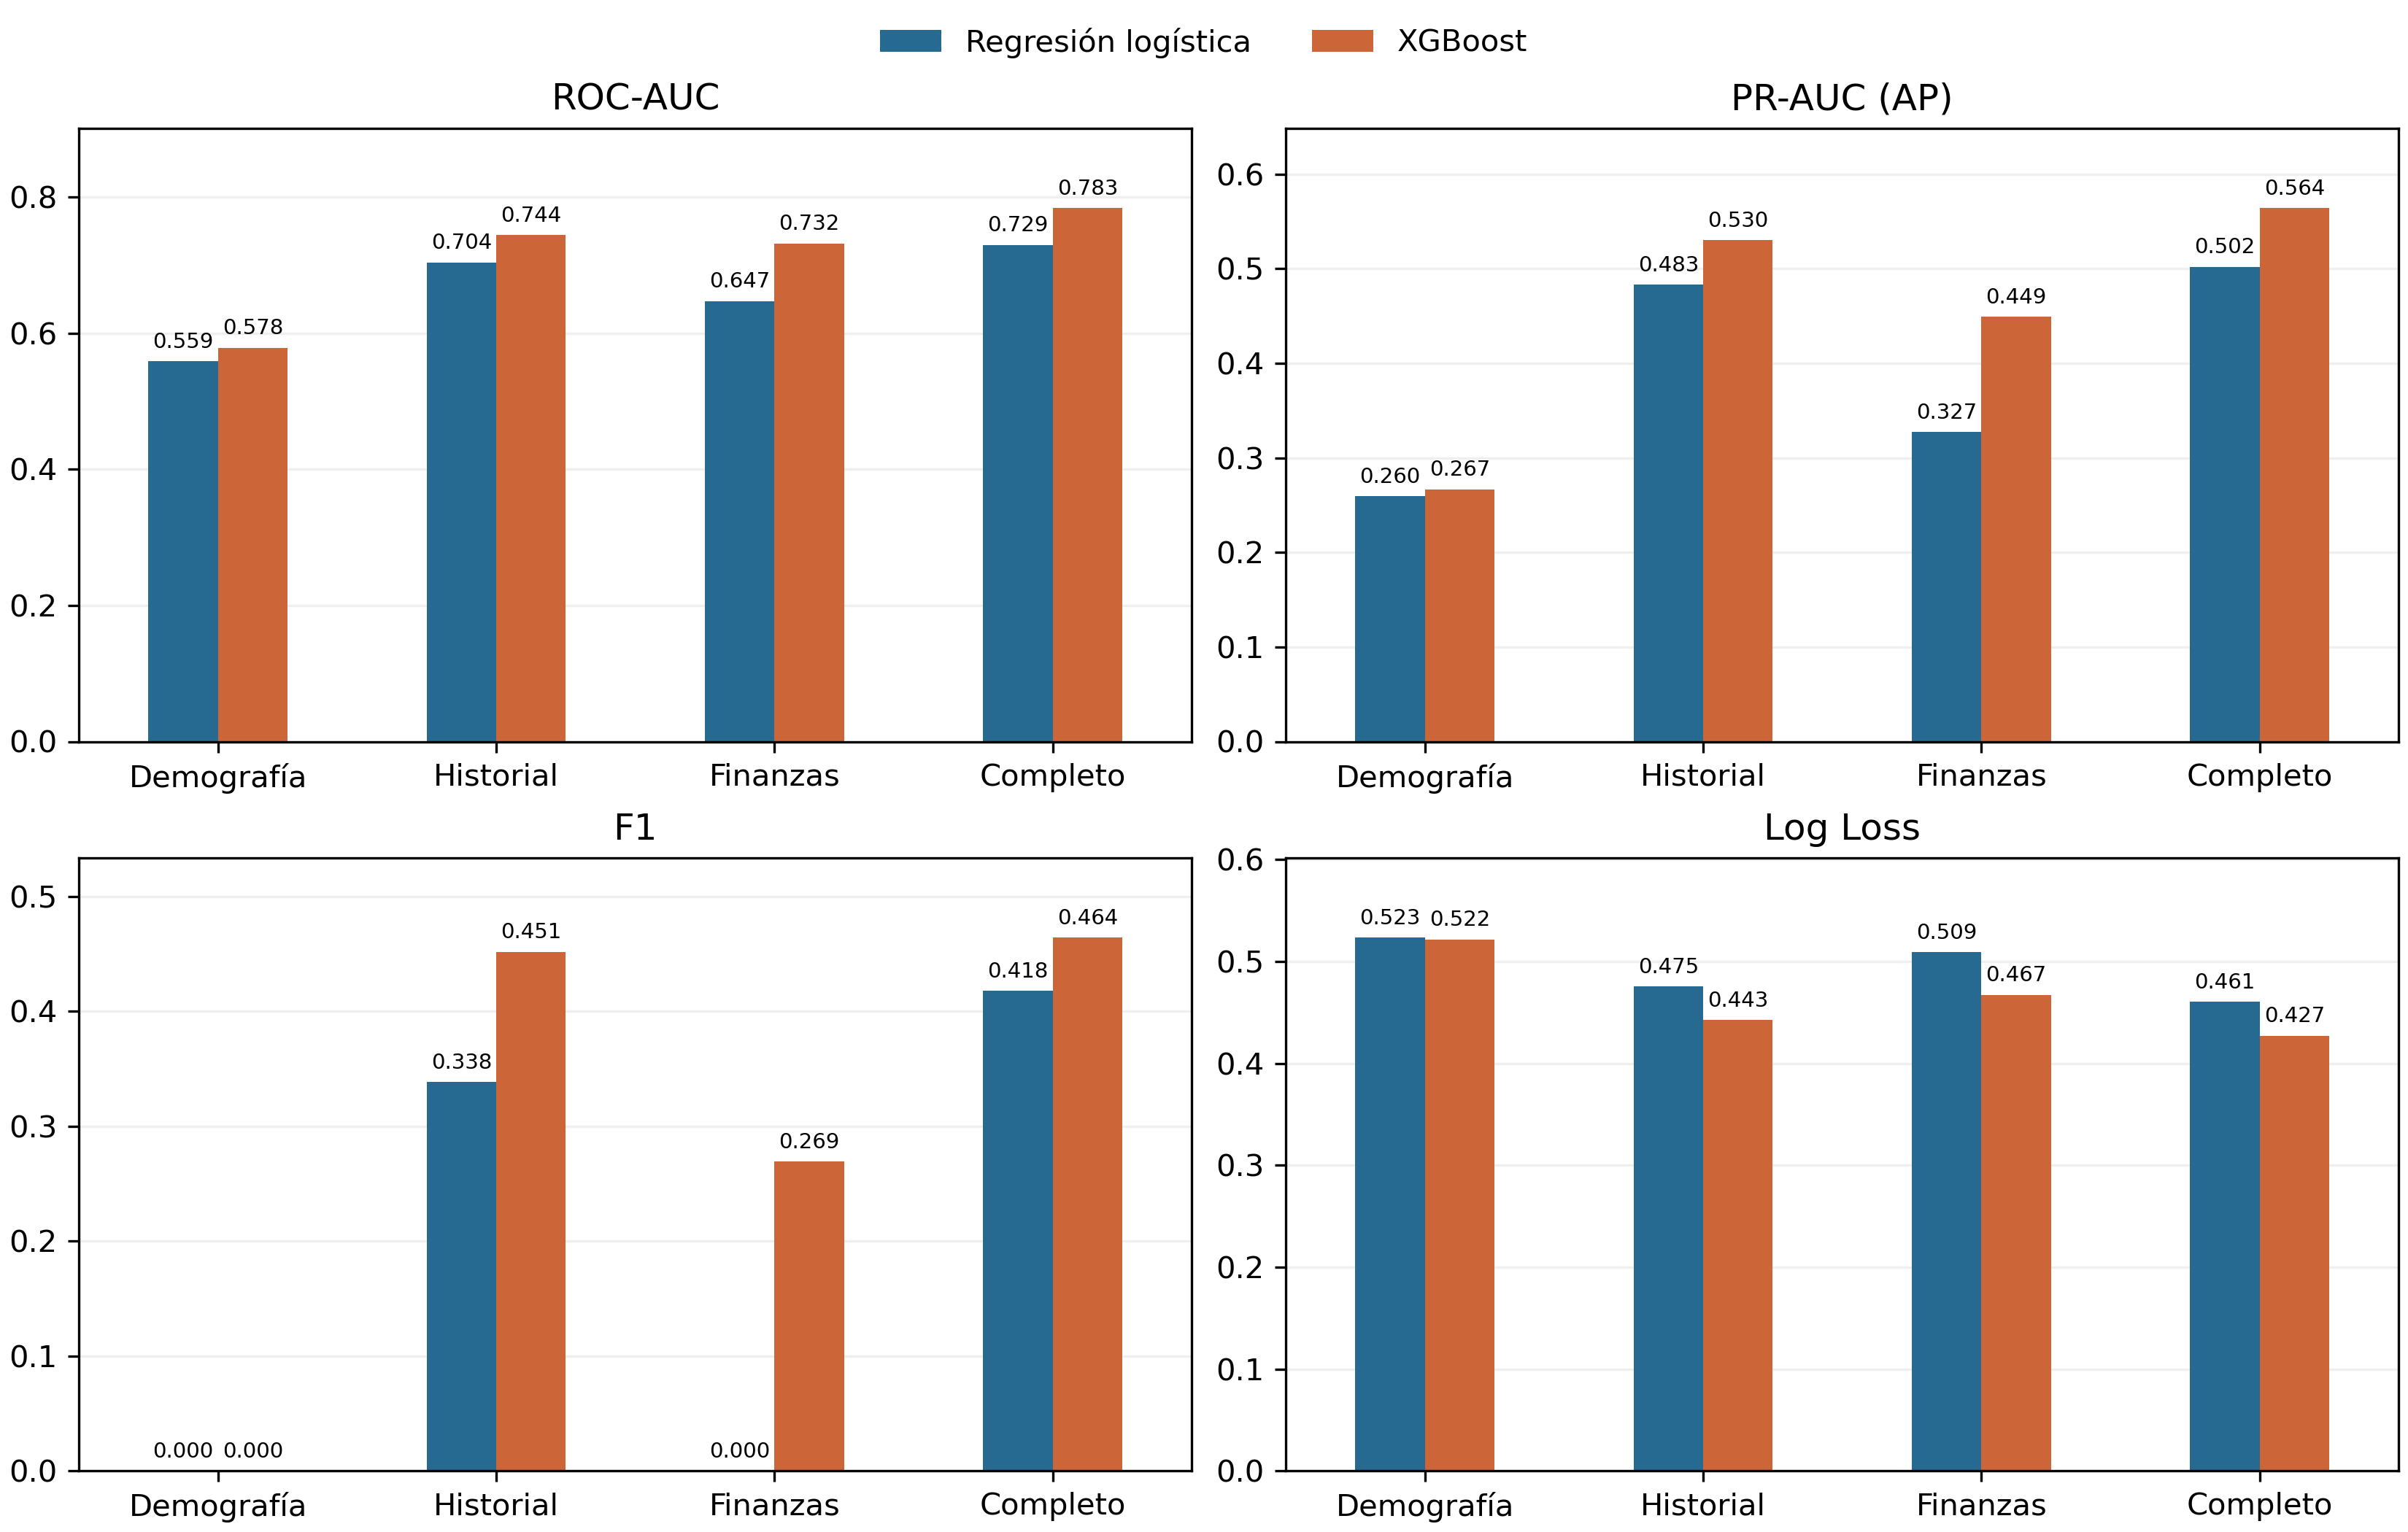
\includegraphics[width=\linewidth,height=.68\textheight,keepaspectratio]{10_ablation_study_comparison.png}\caption{Ablación de bloques en prueba.}\end{figure}

\clearpage
\section{Calibración Probabilística y Cuantificación de Pérdidas Esperadas (\texorpdfstring{$\mathrm{EL}$}{EL})}
Se evaluaron Platt e isotónica con predicciones fuera de pliegue en cinco particiones estratificadas de validación. El menor Brier entre calibradores determinó el ganador; Log Loss resolvía empates. La cruda de XGBoost obtuvo menor Brier que su isotónica también en validación y se reportó como referencia. El calibrador seleccionado se reajustó sobre validación completa. En prueba, la isotónica tiene el menor Brier y ECE uniforme entre candidatos calibrados. El bosque isotónico obtiene menor Log Loss y mayor AP que XGBoost isotónico. La logística isotónica obtiene el menor ECE por cuantiles. El ECE depende de la agrupación y puede cambiar con los empates; el máximo previsto es diez bins. La isotónica produjo dos probabilidades extremas equivocadas en prueba.

\par\medskip\noindent\textbf{Métricas probabilísticas en prueba}

\noindent\reporttable{\begin{tabular}{lrrrrrrr}
\toprule
Modelo & Método & ROC-AUC & AP & Log Loss & Brier & ECE uniforme & ECE cuantiles \\
\midrule
Logística M5 & cruda & 0.7294 & 0.5021 & 0.4606 & 0.1432 & 0.0322 & 0.0313 \\
Árbol & cruda & 0.7628 & 0.5262 & 0.4446 & 0.1385 & 0.0217 & 0.0204 \\
Random Forest & cruda & 0.7817 & 0.5601 & 0.4283 & 0.1344 & 0.0107 & 0.0075 \\
XGBoost & cruda & 0.7834 & 0.5640 & 0.4271 & 0.1341 & 0.0101 & 0.0139 \\
XGBoost & sigmoid & 0.7834 & 0.5640 & 0.4313 & 0.1351 & 0.0206 & 0.0303 \\
XGBoost & isotonic & 0.7804 & 0.5352 & 0.4429 & 0.1346 & 0.0097 & 0.0114 \\
Random Forest & sigmoid & 0.7817 & 0.5601 & 0.4317 & 0.1353 & 0.0201 & 0.0235 \\
Random Forest & isotonic & 0.7804 & 0.5370 & 0.4368 & 0.1348 & 0.0099 & 0.0104 \\
Logística M5 & sigmoid & 0.7294 & 0.5021 & 0.4540 & 0.1423 & 0.0173 & 0.0197 \\
Logística M5 & isotonic & 0.7289 & 0.4843 & 0.4669 & 0.1416 & 0.0113 & 0.0076 \\
\bottomrule\end{tabular}}


\par\medskip\noindent\textbf{Selección de calibrador con validación fuera de pliegue}

\noindent\reporttable{\begin{tabular}{lrrrrr}
\toprule
modelo & método & ROC-AUC & PR-AUC (AP) & Log Loss & Brier Score \\
\midrule
XGBoost & cruda & 0.7796 & 0.5545 & 0.4303 & 0.1355 \\
XGBoost & sigmoid & 0.7789 & 0.5532 & 0.4353 & 0.1366 \\
XGBoost & isotonic & 0.7740 & 0.5396 & 0.4453 & 0.1356 \\
Random Forest & cruda & 0.7754 & 0.5482 & 0.4326 & 0.1363 \\
Random Forest & sigmoid & 0.7748 & 0.5472 & 0.4372 & 0.1374 \\
Random Forest & isotonic & 0.7708 & 0.5338 & 0.4484 & 0.1366 \\
Logística M5 & cruda & 0.7191 & 0.4990 & 0.4631 & 0.1442 \\
Logística M5 & sigmoid & 0.7183 & 0.4968 & 0.4571 & 0.1433 \\
Logística M5 & isotonic & 0.7143 & 0.4836 & 0.4716 & 0.1431 \\
\bottomrule\end{tabular}}


\begin{figure}[htbp]\centering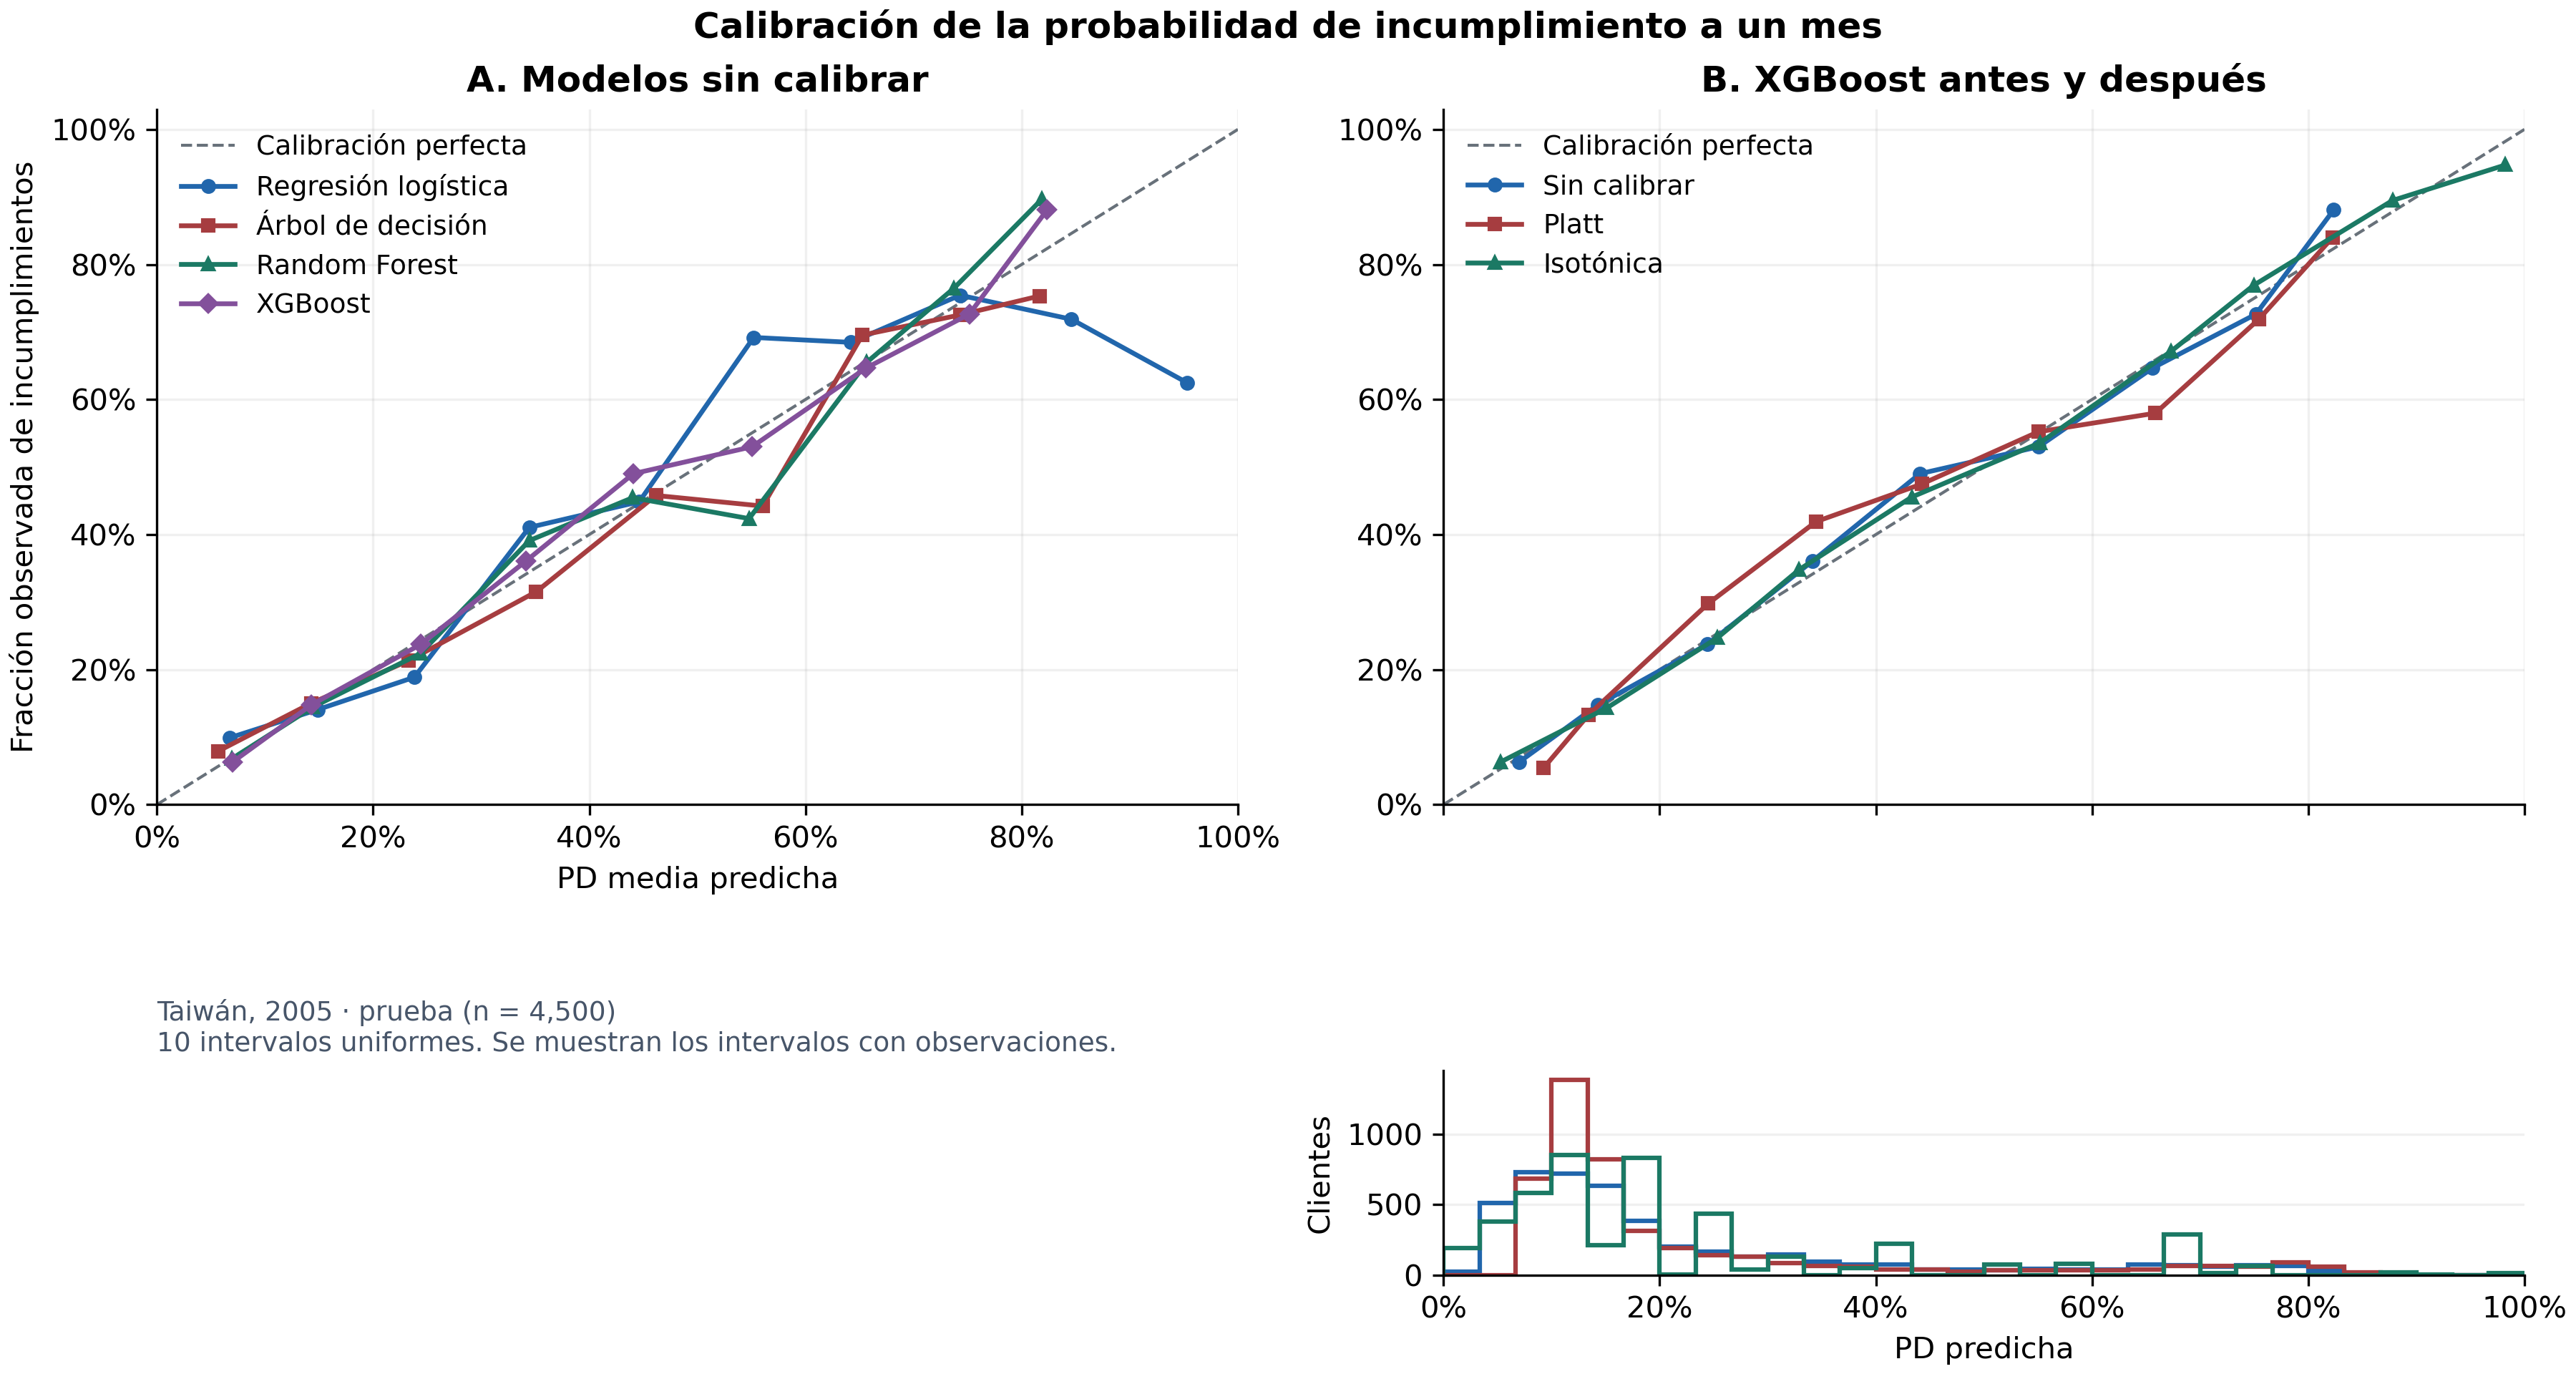
\includegraphics[width=\linewidth,height=.68\textheight,keepaspectratio]{11_calibration_curves_comparison.png}\caption{Comparación de curvas de calibración.}\end{figure}

\[
\mathrm{EL}_{s}=\sum_i \mathrm{PD}_i\,\mathrm{LGD}_{s}\,\mathrm{EAD}_{i,s}.
\]
En base y adverso, el saldo dispuesto se aproxima con $D_i = \max(\text{BILL\_AMT1}_i, 0)$ y la exposición con $D_i + \text{CCF}_s \max(\text{LIMIT\_BAL}_i - D_i, 0)$. En severo, el código usa el límite directamente; para cuentas sobregiradas esto puede reducir su EAD individual frente a la fórmula anterior. En prueba hay 96 facturas negativas y 335 superiores al límite. Las tres simulaciones conservan la misma PD de cada cliente, y sus cambios de EL reflejan los supuestos de exposición y severidad. LGD y CCF son parámetros hipotéticos y EAD una aproximación. Los totales corresponden a los 4\,500 clientes de prueba y están expresados en NTD. La PD media simple aumentó tras calibrar. La PD ponderada por exposición disminuyó en los tres escenarios, con la consiguiente reducción de la EL simulada. La columna de cambio mide la diferencia monetaria entre dos estimaciones que comparten LGD y EAD. El error monetario frente a pérdidas realizadas queda sin identificar.

\par\medskip\noindent\textbf{Escenarios de pérdida esperada en NTD}

\noindent\reporttable{\begin{tabular}{lrrrrrr}
\toprule
Escenario & LGD & CCF & EAD & EL cruda & EL calibrada & Cambio EL \\
\midrule
Base & 0.5500 & 0.5000 & 497,227,726 & 49,306,232 & 48,830,275 & -475,957 \\
Adverso & 0.7000 & 0.7500 & 630,705,184 & 77,515,814 & 76,751,995 & -763,819 \\
Severo & 0.8500 & 1.0000 & 759,657,680 & 111,020,820 & 109,890,095 & -1,130,725 \\
\bottomrule\end{tabular}}


\begin{figure}[htbp]\centering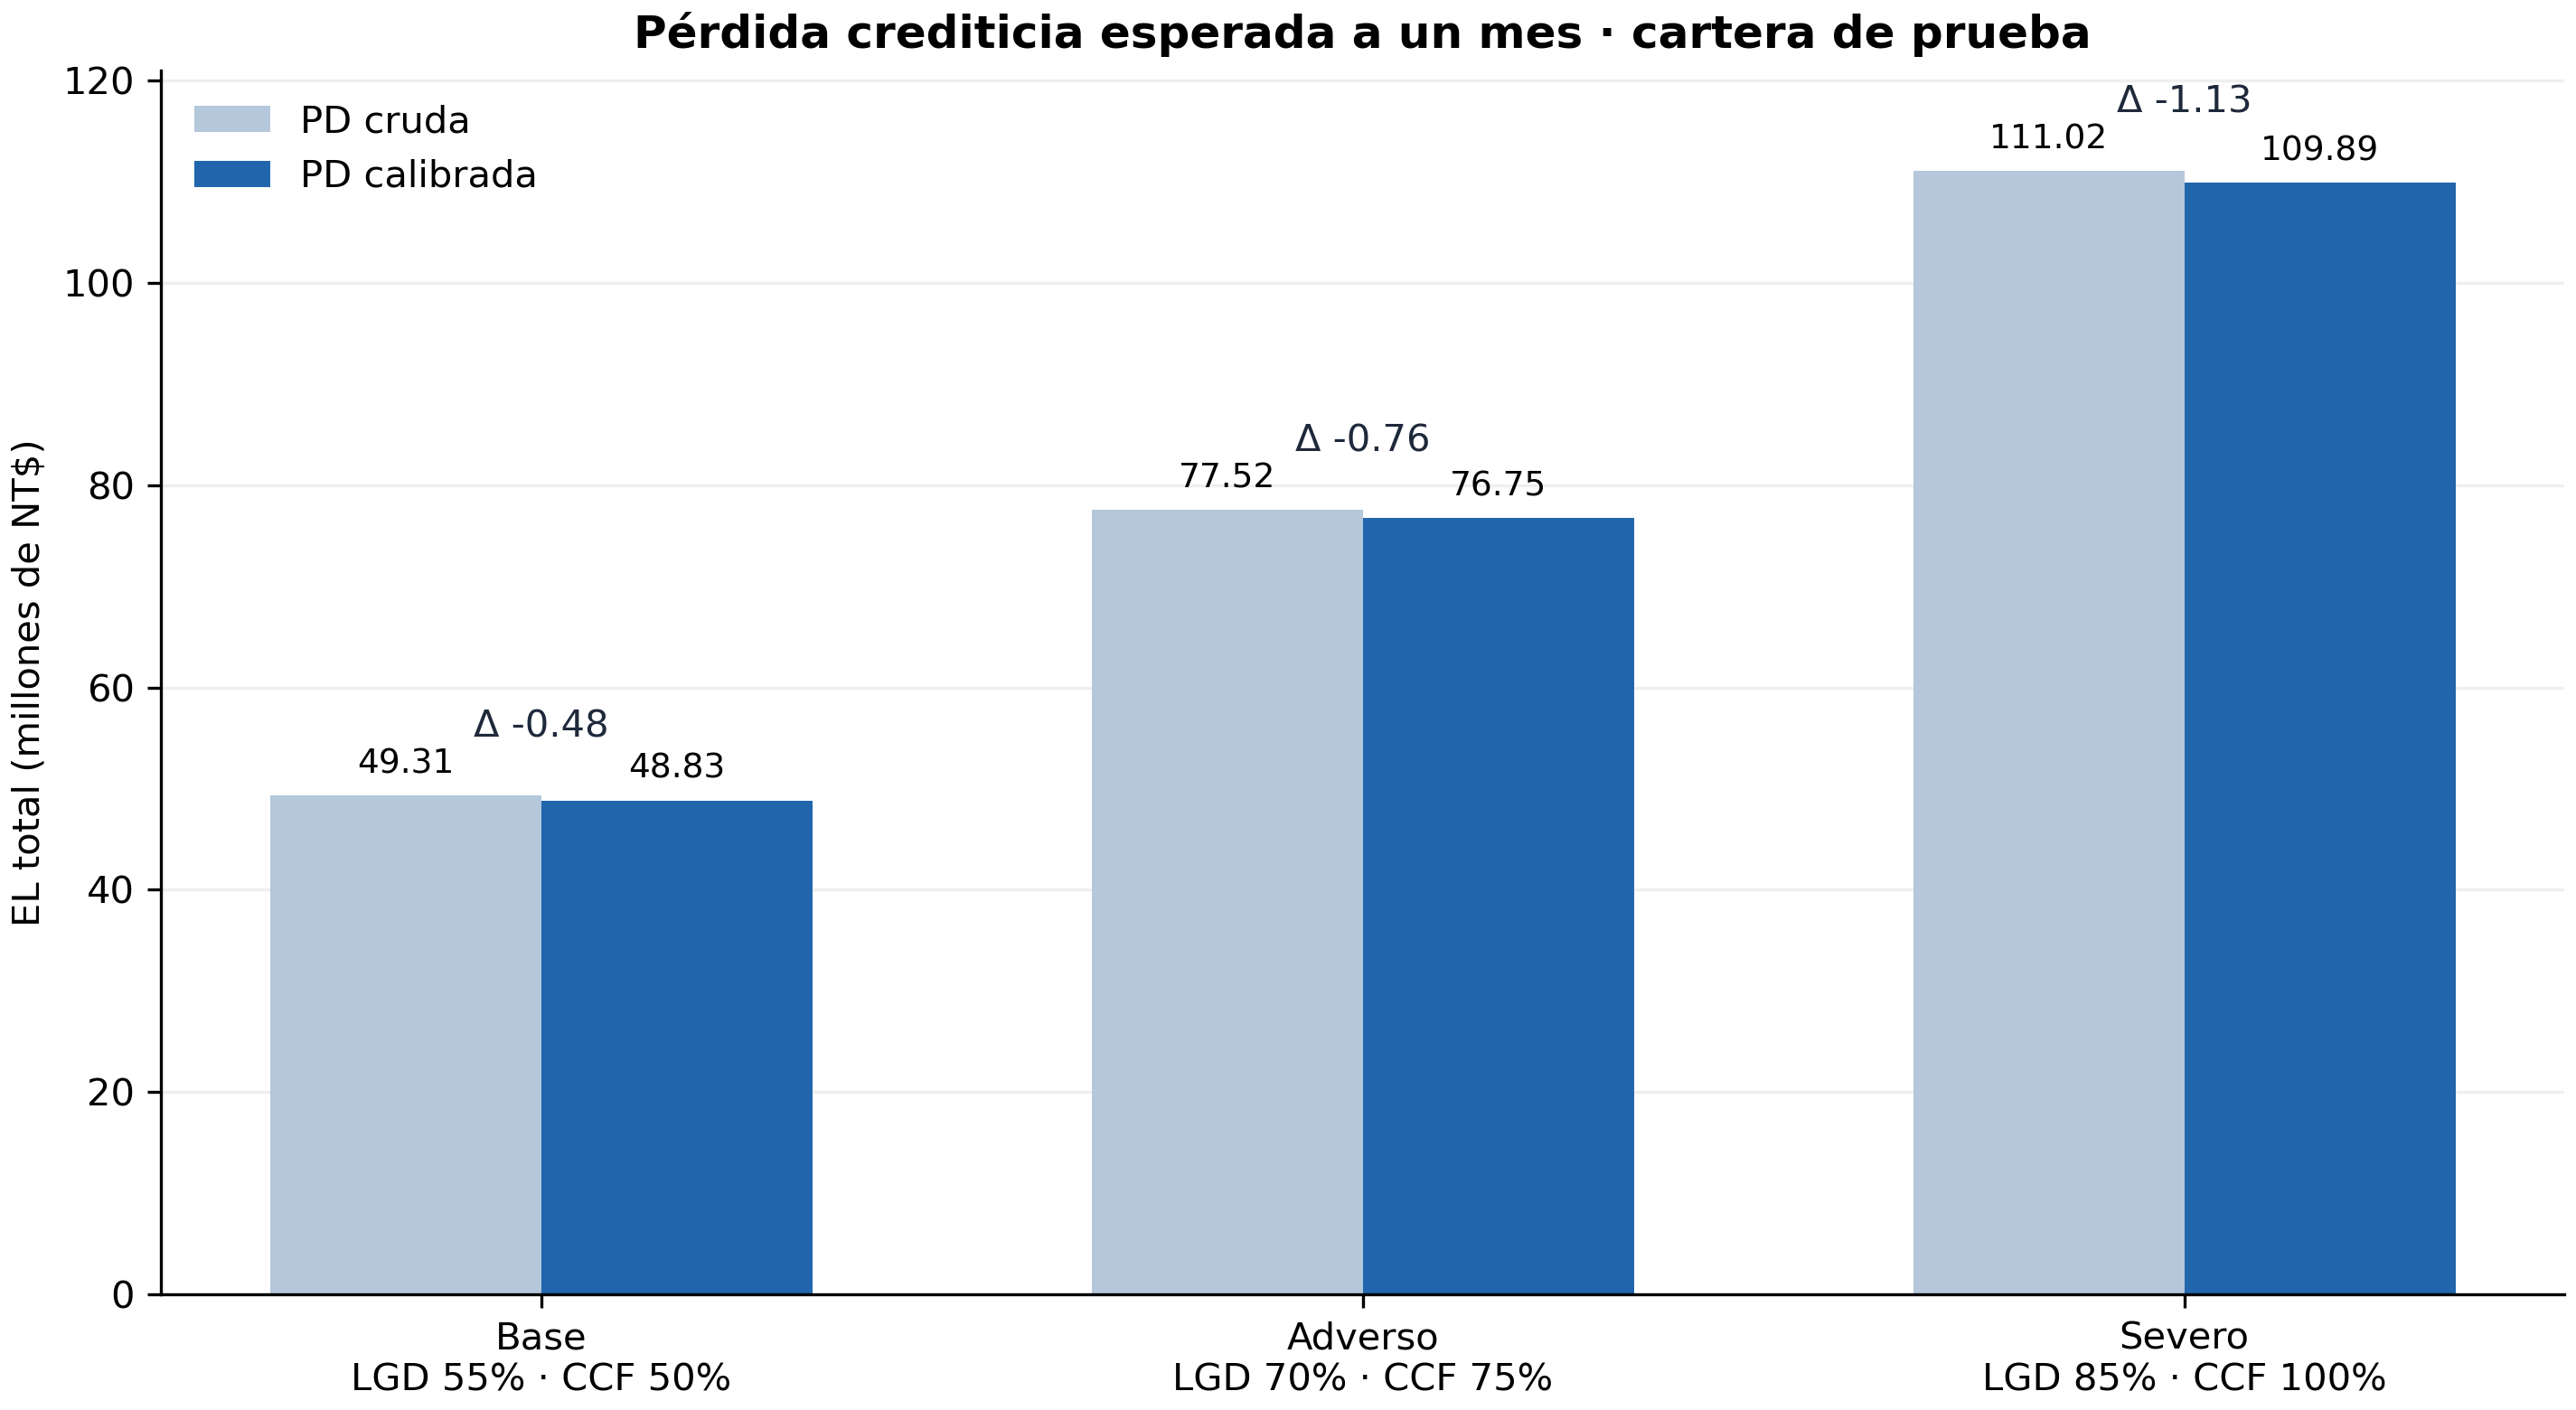
\includegraphics[width=\linewidth,height=.68\textheight,keepaspectratio]{13_expected_loss_scenarios.png}\caption{Pérdida esperada bajo tres escenarios hipotéticos.}\end{figure}

\clearpage
\section{Auditoría por Subgrupos Demográficos y Limitaciones del Estudio}
Se midieron PD media menos frecuencia observada, Brier, FPR entre no incumplidos y FNR entre incumplidos, con un corte común de PD calibrada de 0.2424 heredado del Youden de validación. En la muestra de prueba las decisiones coincidieron con el corte sobre probabilidades crudas. Los hombres muestran subestimación media y mayores FPR y FNR que las mujeres. Secundaria registra la mayor FPR entre niveles de educación con más de dos incumplimientos; el grupo educativo Otros tiene dos incumplimientos y resultados inestables. En estado civil, Otros tiene el mayor sesgo positivo y 9 incumplimientos. En edad, el grupo mayor de 45 presenta subestimación y la FPR más alta; el de 30--45 tiene la FNR más alta. Son comparaciones descriptivas sin intervalos ni ajuste por composición. La calibración media evalúa un aspecto del desempeño y la equidad requiere evidencia adicional.

\par\medskip\noindent\textbf{Desempeño en prueba por grupo}

\noindent\reporttable{\begin{tabular}{lrrrrrrrr}
\toprule
Variable y grupo & n & Eventos & Obs. & PD media & Sesgo & Brier & FPR & FNR \\
\midrule
\texttt{SEX} Hombres & 1766 & 448 & 0.2537 & 0.2333 & -0.0204 & 0.1545 & 0.2451 & 0.3571 \\
\texttt{SEX} Mujeres & 2734 & 548 & 0.2004 & 0.2136 & 0.0131 & 0.1217 & 0.2113 & 0.3376 \\
\texttt{EDUCATION} Posgrado & 1580 & 320 & 0.2025 & 0.1922 & -0.0103 & 0.1269 & 0.1952 & 0.4031 \\
\texttt{EDUCATION} Universidad & 2086 & 477 & 0.2287 & 0.2370 & 0.0083 & 0.1356 & 0.2318 & 0.3040 \\
\texttt{EDUCATION} Secundaria & 766 & 197 & 0.2572 & 0.2494 & -0.0078 & 0.1574 & 0.2900 & 0.3553 \\
\texttt{EDUCATION} Otros & 68 & 2 & 0.0294 & 0.0995 & 0.0701 & 0.0257 & 0.0152 & 0.5000 \\
\texttt{MARRIAGE} Casado & 2063 & 498 & 0.2414 & 0.2270 & -0.0144 & 0.1412 & 0.2288 & 0.3474 \\
\texttt{MARRIAGE} Soltero & 2383 & 489 & 0.2052 & 0.2153 & 0.0101 & 0.1291 & 0.2165 & 0.3476 \\
\texttt{MARRIAGE} Otros & 54 & 9 & 0.1667 & 0.2659 & 0.0993 & 0.1236 & 0.3778 & 0.2222 \\
\texttt{AGE} \textless{}30 & 1414 & 314 & 0.2221 & 0.2329 & 0.0108 & 0.1331 & 0.2227 & 0.3089 \\
\texttt{AGE} 30–45 & 2354 & 488 & 0.2073 & 0.2077 & 0.0004 & 0.1307 & 0.2165 & 0.3709 \\
\texttt{AGE} \textgreater{}45 & 732 & 194 & 0.2650 & 0.2426 & -0.0224 & 0.1500 & 0.2528 & 0.3454 \\
\bottomrule\end{tabular}}


\begin{figure}[htbp]\centering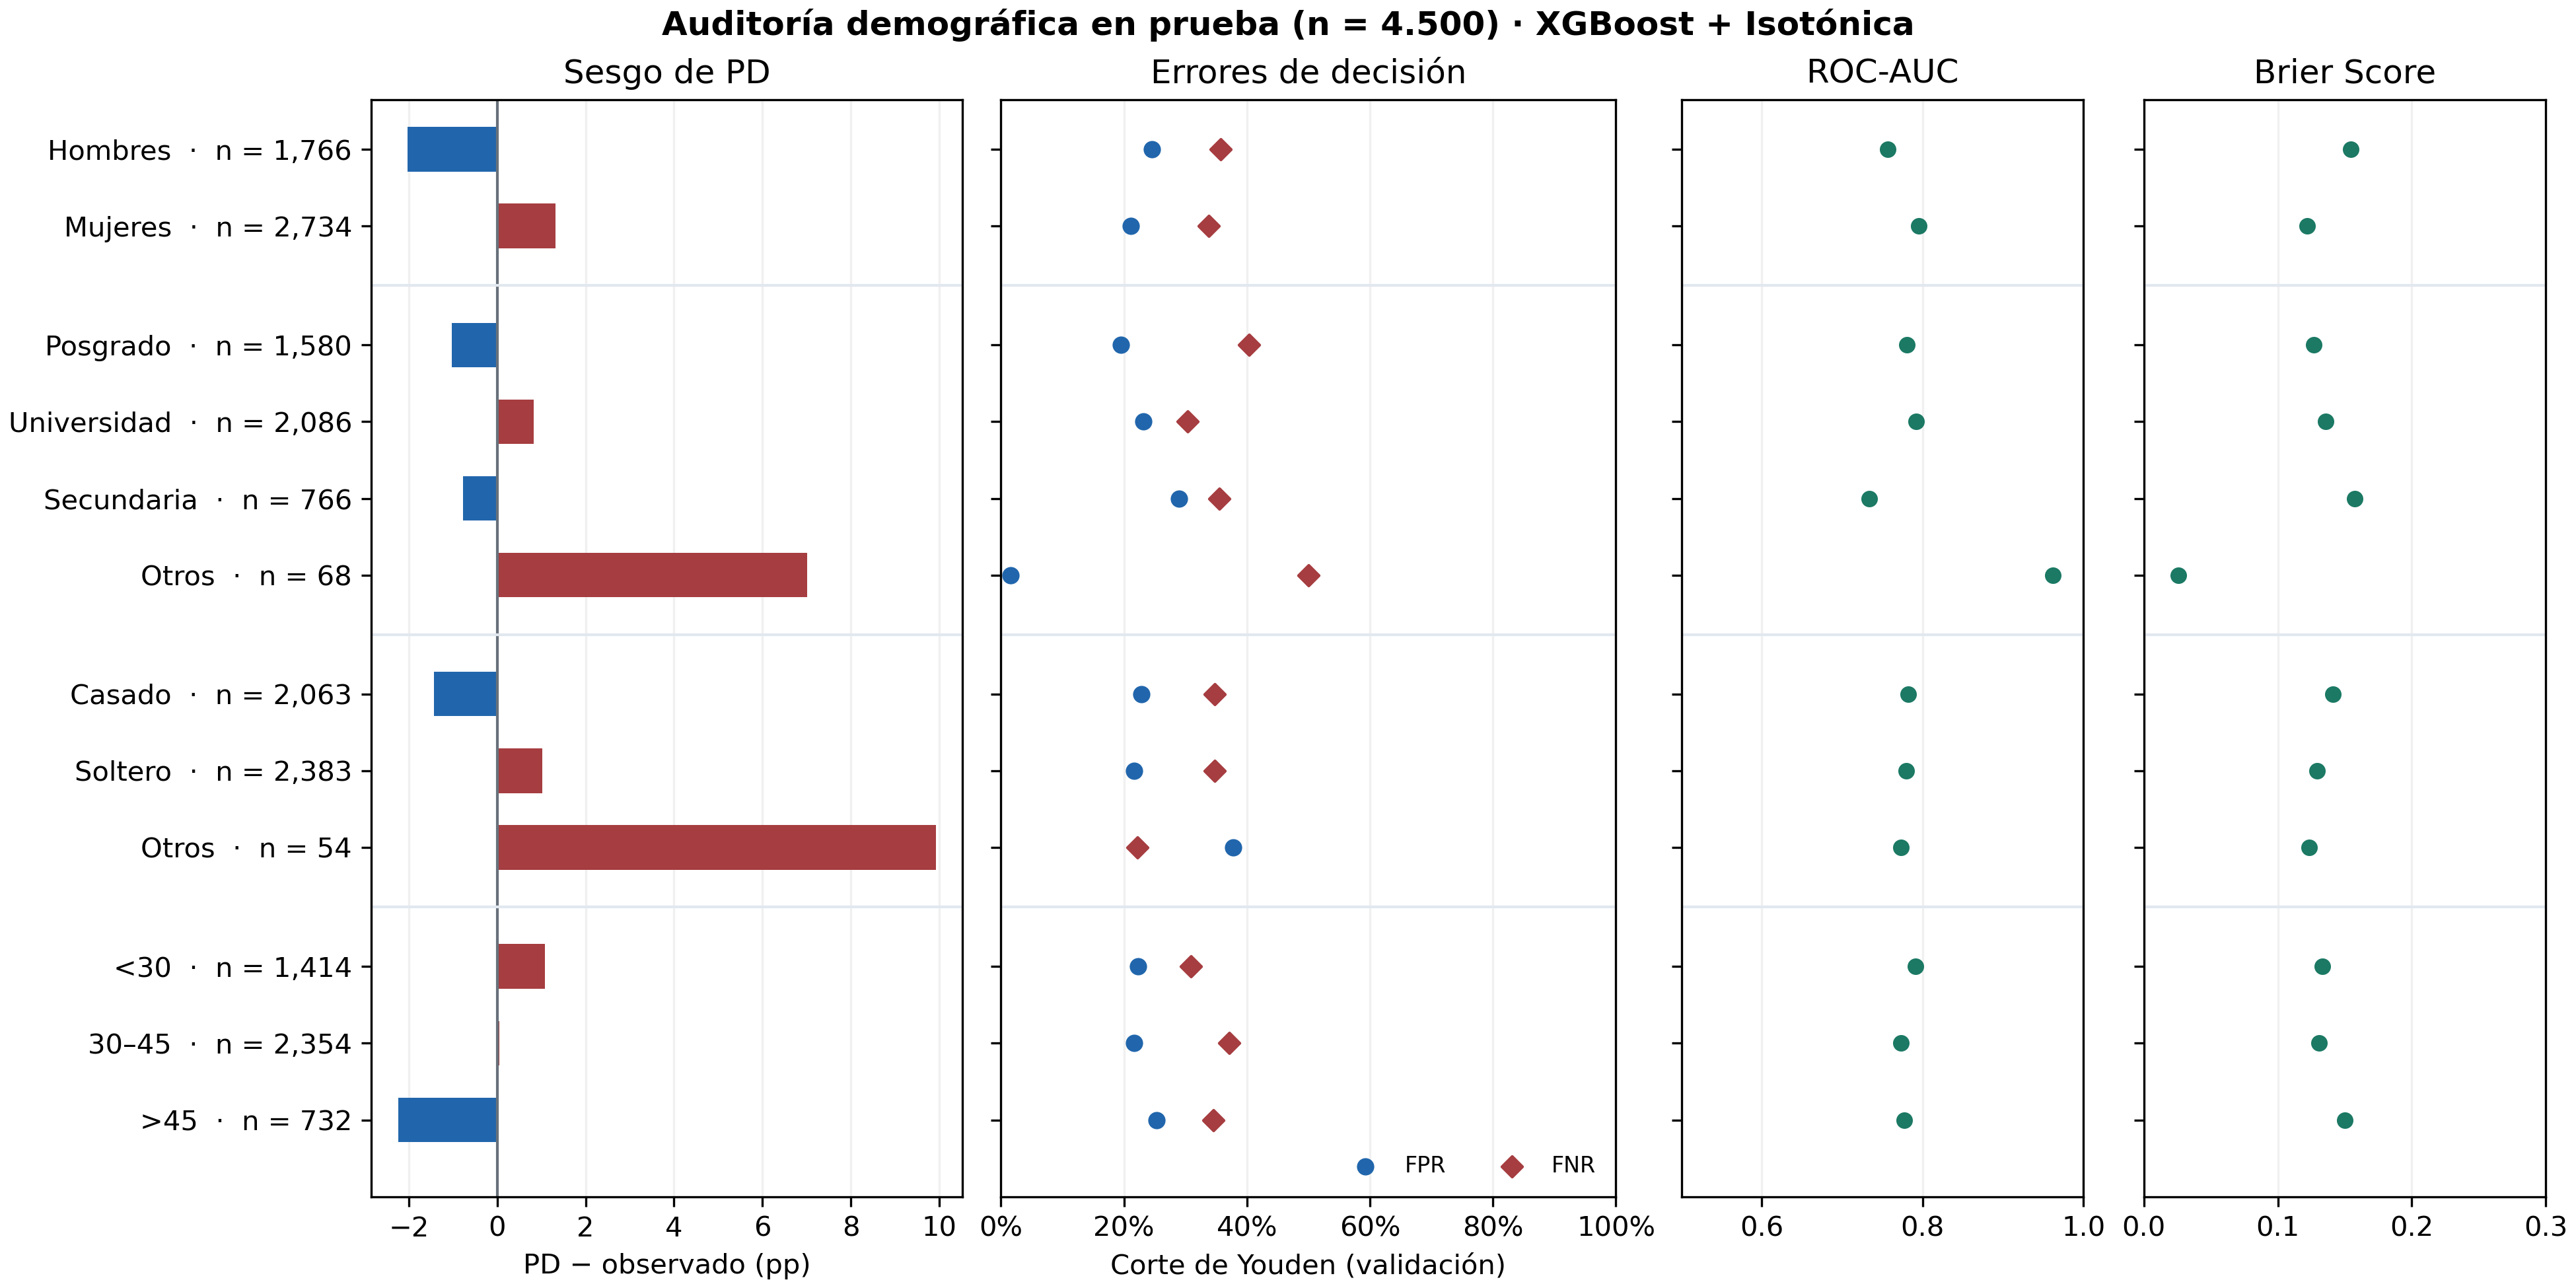
\includegraphics[width=\linewidth,height=.68\textheight,keepaspectratio]{12_demographic_fairness_audit.png}\caption{Calibración media y tasas de error por grupo.}\end{figure}

El corte transversal abarca clientes de Taiwán con historial de abril a septiembre de 2005. Las asociaciones observacionales están sujetas a confusión, selección y especificación. La identificación de efectos causales requiere variación exógena o un diseño con supuestos de identificación explícitos. La aplicación a Colombia exige datos locales, validación externa y recalibración o reestimación. La base carece de datos sobre recuperaciones y exposición observada al incumplimiento. LGD y EAD se cuantifican mediante supuestos de escenario.

\clearpage
\section{Conclusiones y Trabajo Futuro}
M5 ofrece una especificación interpretable con control de colinealidad en los saldos y evidencia de interacciones en el logit. El historial de pago aporta la mayor señal incremental para predecir el incumplimiento. La evaluación de calibración muestra que los criterios de selección pueden divergir: la isotónica reduce el ECE de XGBoost y la PD cruda conserva mejores puntuaciones probabilísticas en prueba.

Una extensión empírica evaluaría estabilidad y calibración en cohortes colombianas independientes. También estimaría LGD y EAD con registros de recuperaciones y disposición efectiva al incumplir, y cuantificaría la incertidumbre de las diferencias de desempeño entre subgrupos.

\begin{thebibliography}{9}
\bibitem{uci} Yeh, I. Default of Credit Card Clients. UCI Machine Learning Repository. \href{https://doi.org/10.24432/C55S3H}{DOI 10.24432/C55S3H}.
\bibitem{yeh} Yeh, I.-C. y Lien, C.-H. (2009). The comparisons of data mining techniques for the predictive accuracy of probability of default of credit card clients. \emph{Expert Systems with Applications}. \href{https://doi.org/10.1016/j.eswa.2007.12.020}{DOI 10.1016/j.eswa.2007.12.020}.
\end{thebibliography}
\end{document}
